\documentclass[aps,pra,superscriptaddress,floatfix,longbibliography,twocolumn]{revtex4-2}
\usepackage{graphicx}
\usepackage{amsmath,amssymb,amsthm}
\usepackage{bm}
\usepackage{algpseudocode}
\usepackage[colorlinks=true,linkcolor=blue,citecolor=blue,urlcolor=blue]{hyperref}
\bibliographystyle{apsrev4-2}
\newcommand{\bx}{{\bf x}}
\newcommand{\bu}{{\bf u}}
\newcommand{\by}{{\bf y}}
\newcommand{\bb}{{\bf b}}
\newcommand{\bc}{{\bf c}}
\newcommand{\bs}{{\bf s}}
\newcommand{\bv}{{\bf v}}
\newcommand{\bz}{{\bf z}}
\newcommand{\bw}{{\bf w}}
\newcommand{\be}{{\bf e}}
\newtheorem{proposition}{Proposition}
\newtheorem{theorem}{Theorem}
\newtheorem{lemma}{Lemma}

\begin{document}
\title{Selected input--output responses of large linear systems from divided-difference walk sums}
\author{Amir Kalev}
\affiliation{Information Sciences Institute, University of Southern California, Arlington, VA 22203, USA}
\author{Ivan Bermejo-Moreno}
\affiliation{Department of Aerospace and Mechanical Engineering, Viterbi School of Engineering, University of Southern California, Los Angeles, CA 90089, USA}
\author{Itay Hen}
\email{itayhen@isi.edu}
\affiliation{Information Sciences Institute, University of Southern California, Marina del Rey, California 90292, USA}
\affiliation{Department of Physics and Astronomy and Center for Quantum Information Science \& Technology, University of Southern California, Los Angeles, California 90089, USA}

\begin{abstract}
We consider the computation of a few input--output responses $\by=C\bx$ of a linear time-invariant system $\dot\bx=A\bx+B\bu$ whose state dimension is too large for the state vector to be stored, or large enough that storing it dominates the cost. Starting from the off-diagonal expansion of the matrix exponential, in which an entry of $e^{tA}$ is a sum over walks on the graph of couplings weighted by divided differences of the exponential at the visited diagonal entries, we derive the walk form of forced responses, a divided-difference kernel that returns each walk's temporal factor on a whole time grid, and bounds that certify the truncation error of pruned traversals in terms of the ratio $\mu$ of couplings to local decay rates. The same bounds certify local truncations to a ball or to an adaptively grown set of states. In a C++ implementation the whole process used a few megabytes for implicitly specified networks with up to $2^{64}$ states. With the same distance information for all methods and the walk sum charged for its full threshold search, the walk sum reached a certified truncation error of $10^{-4}$ on a random network of degree 32 with $\mu=0.57$ in 2.4~s and 6~MB, against 13~s and 53~MB for the adaptive local truncation. Over three graph seeds and three actuator locations per seed, at degrees 16 and 32, the adaptive truncation took 1.5 to 19 times longer. The runtime advantage also held in the tested degree-16 transfer responses between separated actuator and sensor states. On lattices local truncation was faster by orders of magnitude, and the cost of the walk sum grows steeply as $\mu$ approaches one.
\end{abstract}
\maketitle

\section{Introduction}\label{sec:intro}

Many questions asked of a large linear dynamical system concern a handful of its outputs. A thermal model of a chip is probed at a few sensor locations while a few heaters are driven; a networked system is excited at a few driver nodes and observed at a few others~\cite{liu2011,pasqualetti2014,mesbahi2010}; a stochastic model is queried for the probability of a few configurations. In state-space form the object of interest is $\by(t)=C\bx(t)$ for $\dot\bx=A\bx+B\bu$, with $C$ and $B$ having few rows and columns, and the state dimension $N$ may be far larger than anything that has to be reported.

Standard methods nevertheless work with the full state. Time integrators propagate $\bx(t)$. The scaled Taylor method of Al-Mohy and Higham~\cite{almohy2011} and Krylov methods~\cite{hochbruck1997,sidje1998} compute the action $e^{tA}\bv$ and need a few, or $m+1$, vectors of length $N$, in addition to $A$ itself; limited-memory variants reduce the multiple but not the scaling~\cite{guttel2020}. None of these stores $e^{tA}$, and for moderate $N$ they are the right tools. They become the wrong tools when the state vector itself does not fit, which happens for implicitly specified models with astronomically many states, or when memory is the binding constraint and only a few numbers are wanted. Local methods restrict the computation to a neighborhood of the inputs, as in the finite state projection for master equations~\cite{munsky2006} or push methods for exponentials of graph matrices~\cite{kloster2014,gleich2015}, and their memory is the size of that neighborhood. Model reduction~\cite{antoulas2005} amortizes an offline cost over many queries and is a different trade.

Barash, G\"uttel and Hen~\cite{barash2022} showed that an individual entry of a matrix function can be evaluated as a sum over walks on the graph of off-diagonal couplings, each walk weighted by a divided difference of the function at the diagonal entries it visits, with memory that does not grow with $N$. This is the off-diagonal (permutation-matrix) expansion developed for quantum Monte Carlo~\cite{albash2017,gupta2020pmr}; related path-sum constructions appear in Refs.~\cite{giscard2013,giscard2015,gorban2011}. Here we develop this representation for linear time-invariant systems, homogeneous and forced, and ask a question with a measurable answer: when can selected input--output responses be computed from walk sums with working memory independent of $N$, with a certified truncation error and at a practical cost, and how does that compare with the alternatives, in particular with local methods that use the same error bounds?

What is established and what is new should be kept apart. The walk expansion of $e^{tA}$ and its depth-first evaluation with incremental divided differences are those of Ref.~\cite{barash2022}. That an exponential forcing can be absorbed by enlarging the system is classical~\cite{vanloan1978,almohy2011}. The contributions of this paper are the following. (i) A linear input--output calculus in walk form: responses to exponential-polynomial inputs append a block of confluent nodes to each walk (Proposition~\ref{prop:forcing}), delayed and piecewise inputs are handled through a truncated-power basis without reconstructing the state at breakpoints, and all input patterns and observation times are obtained from one traversal. (ii) An output-oriented algorithm: backward enumeration from the sensors, lazy evaluation of the temporal factors, and a divided-difference kernel that returns a whole time grid by exact stepping of each walk's bidiagonal system; it handles repeated and clustered nodes without special cases, uses only nonnegative quantities in its squaring and stepping stages for real nodes, and was tested for complex ones. (iii) Error control: uniform-in-time componentwise bounds in terms of the comparison matrix $H^{-1}|R|$ that relates couplings to local decay rates, finite-horizon bounds for the general case, and an a posteriori certificate of the truncation error that accompanies subtree pruning, together with an accounting of the floating-point errors that the certificate does not cover. (iv) The same bounds certify local truncations of the system, a ball around the inputs and an adaptively grown set (Proposition~\ref{prop:local}), which gives local comparators with the same guarantee. (v) A measured assessment of memory and time from scratch against global and local methods on networks of up to $2^{64}$ states, with shared distance information, including the regimes where the walk sum loses. Appendix~\ref{app:td} records the extension to generators with exponential time dependence.

The measurements support three statements. First, the method does what its memory accounting promises: a few megabytes for the whole process, flat in $N$, for responses with a certified truncation error of systems whose state could not be stored. Second, on locally tree-like coupling graphs of degree 16 and 32 it was also the fastest of the certified methods we tested, against the uniform ball and against the adaptive set, given the same distance information, at every target that any of them reached; its peak memory stayed between 4.5 and 6.1~MB (7.2~MB with the larger distance map used for separated sensors) while the local methods needed up to 3~GB. The advantage held over three graph seeds and three actuator locations per seed for each degree, by factors of 1.5 to 19 in time against the adaptive set. At degree 4 all methods finished in tens of milliseconds and the adaptive set was marginally faster. Third, the walk sum loses, by orders of magnitude, on lattices, where many walks revisit the same states and a local state vector merges them, and when the coupling-to-decay ratio approaches or exceeds one, as in strongly nonnormal transport. Section~\ref{sec:numerics} documents these statements. In short, for selected responses of implicitly represented systems, certified walk pruning replaces the retained state vector of a local method by a small traversal workspace, and on high-degree tree-like coupling graphs the lazy evaluation of temporal factors makes it faster as well; the $2^{64}$-state examples illustrate the access model rather than the source of the advantage.

%% ---------------------------------------------------------------------------------------------
\section{Problem and access model}\label{sec:problem}

We consider the continuous-time linear time-invariant system
\begin{equation}\label{eq:lti}
\begin{aligned}
\dot\bx(t)&=A\bx(t)+B\bu(t),\qquad \bx(0)=\bx_0,\\
\by(t)&=C\bx(t)+F\bu(t),
\end{aligned}
\end{equation}
with $A\in\mathbb{C}^{N\times N}$, $B\in\mathbb{C}^{N\times m}$, $C\in\mathbb{C}^{p\times N}$ and direct feedthrough $F\in\mathbb{C}^{p\times m}$. The target regime has $m,p\ll N$, sparse rows of $C$ and sparse columns of $B$ and $\bx_0$. Real systems are the main special case; complex arithmetic enters only through complex diagonal entries, complex couplings, or complex input rates. A prescribed forcing $\bb(t)$ is the case $B\bu(t)=\bb(t)$.

The quantities we compute are, on a uniform grid $t_k=k\,\Delta t$, $k=0,\dots,T$:
(i) zero-input responses $C e^{tA}\bx_0$;
(ii) entries of the impulse-response kernel $K(t)=Ce^{tA}B$;
(iii) forced responses for inputs that are exponential polynomials, their delayed and piecewise combinations, and sinusoids; and
(iv) batches of such inputs and observation times evaluated in a single pass.
Forward response evaluation is the only task addressed. Controller synthesis, closed-loop operation and controllability analysis are outside the scope of this paper.

\paragraph*{Access model.} Write $A=D+R$ with $D=\mathrm{diag}(d_1,\dots,d_N)$ and $R$ zero on the diagonal. The directed edge $j\to i$ carries the weight $R_{ij}$. The algorithm needs three oracles: the diagonal entry $d_j$; the list of incoming edges of a state $j$, that is, the nonzero entries of row $j$ of $R$; and entry access to the supports of the rows of $C$ and the columns of $B$ and $\bx_0$. Row access is what a compressed-sparse-row matrix provides, so no transpose is formed. We distinguish two settings. In the \emph{explicit} setting $A$ is stored, and its storage is part of the memory bill of every method. In the \emph{implicit} setting the oracles are local formulas, as for the structured models of Sec.~\ref{sec:numerics}, and nothing of size $N$ is stored. The cost of an oracle call is taken to be independent of $N$; for the implicit models used here it is a few hash evaluations. The error bounds of Sec.~\ref{sec:error} also need a few global constants (the largest real part of a diagonal entry, the largest coupling row sum, the comparison ratio $\mu$ defined there). For an explicit model they come from one pass over $A$; for an implicit model they follow either from the ranges of the model parameters, which gives valid upper bounds at no cost, or from a streaming pass over all states in $O(N)$ time and $O(1)$ memory. Optional distance information (a lower bound on the number of hops from the input support to a state) sharpens the truncation certificates of Sec.~\ref{sec:error}; it is analytic for lattices and otherwise obtained by a breadth-first search whose memory we report separately.

%% ---------------------------------------------------------------------------------------------
\section{Walk-sum representation of input--output responses}\label{sec:representation}

\subsection{Divided differences}
For complex nodes $z_0,\dots,z_q$ (repetitions allowed) let $f_t[z_0,\dots,z_q]$ denote the divided difference of $z\mapsto e^{tz}$. Repeated nodes are part of the definition, not an exceptional case: with $\Gamma$ a contour enclosing all nodes,
\begin{equation}\label{eq:dd_contour}
f_t[z_0,\dots,z_q]=\frac{1}{2\pi i}\oint_\Gamma \frac{e^{tz}\,dz}{\prod_{r=0}^q (z-z_r)} .
\end{equation}
We use the following standard facts~\cite{deboor2005,higham2008,opitz1964}.
\begin{enumerate}
\item[(D1)] Hermite--Genocchi: $f_t[z_0,\dots,z_q]=t^q\int_{\Sigma_q}\exp\!\big(t\sum_r\sigma_r z_r\big)\,d\sigma$, where $\Sigma_q$ is the standard simplex with total measure $1/q!$.
\item[(D2)] Laplace transform: $\int_0^\infty e^{-st}f_t[z_0,\dots,z_q]\,dt=\prod_r (s-z_r)^{-1}$ for $\mathrm{Re}\,s>\max_r\mathrm{Re}\,z_r$.
\item[(D3)] Shift: $f_t[z_0+c,\dots,z_q+c]=e^{ct}f_t[z_0,\dots,z_q]$.
\item[(D4)] Opitz: if $Z$ is lower bidiagonal with diagonal $(z_0,\dots,z_q)$ and unit subdiagonal, then $(e^{tZ})_{rm}=f_t[z_m,\dots,z_r]$ for $r\ge m$.
\end{enumerate}
From (D1), $|f_t[z]|\le f_t[\mathrm{Re}\,z]\le e^{\omega t}t^q/q!$ with $\omega=\max_r\mathrm{Re}\,z_r$; for real nodes $f_t$ is positive and nondecreasing in each node.

\subsection{The walk expansion}
A walk $p=(j_0,j_1,\dots,j_q)$ of length $|p|=q$ is a sequence of states with $R_{j_rj_{r-1}}\neq0$. Its weight and node list are
\begin{equation}
w_p=\prod_{r=1}^q R_{j_r j_{r-1}},\qquad \mathcal{D}_p=(d_{j_0},\dots,d_{j_q}).
\end{equation}
The coefficient of each hop is the matrix entry in the row of its destination, $R_{j_rj_{r-1}}$, consistent with $DP\,\be_j=D_{kk}\be_k$ when a permutation $P$ maps $\be_j$ to $\be_k$. The length-zero walk $p=(i)$ contributes $\delta_{ij}e^{td_i}$.

\begin{proposition}[walk expansion]\label{prop:walk}
For every $t\ge0$,
\begin{equation}\label{eq:walk}
(e^{tA})_{ij}=\sum_{q=0}^{\infty}\ \sum_{p:\,j\to i,\ |p|=q} w_p\, f_t[\mathcal{D}_p],
\end{equation}
and the double series converges absolutely, $\sum_q\sum_{p:j\to i,|p|=q}|w_p|\,|f_t[\mathcal{D}_p]|\le e^{\omega t}e^{\beta t}$ with $\omega=\max_j\mathrm{Re}\,d_j$ and $\beta=\max_i\sum_j|R_{ij}|$.
\end{proposition}
\begin{proof}
For $\mathrm{Re}\,s>\omega+\beta$ the Neumann series $(sI-A)^{-1}=\sum_{q\ge0}[(sI-D)^{-1}R]^q(sI-D)^{-1}$ converges in the row-sum norm, and the $(i,j)$ entry of its $q$-th term is $\sum_{p:j\to i,|p|=q}w_p\prod_r(s-d_{j_r})^{-1}$. By (D2) each product is the Laplace transform of $f_t[\mathcal{D}_p]$. The bound $|f_t[\mathcal{D}_p]|\le e^{\omega t}t^q/q!$ and $\sum_{|p|=q}|w_p|\le\beta^q$ give absolute convergence of the time-domain series, uniformly for $t$ in compact sets, which justifies termwise transformation; uniqueness of the Laplace transform gives \eqref{eq:walk}.
\end{proof}
This expansion and its use for single entries of $f(A)$ are due to Barash, G\"uttel and Hen~\cite{barash2022}, building on the off-diagonal series of Refs.~\cite{albash2017,gupta2020pmr}; the proof above handles complex and repeated nodes without separate limiting arguments. Along each walk the diagonal dynamics is integrated exactly, which is why the number of coupling events needed (the walk length) is governed by the size of the couplings relative to the local decay rates, not by $\|A\|$. Exact integration of the diagonal does not by itself make a stiff problem easy: what matters is how many coupling events contribute, which Sec.~\ref{sec:error} bounds.

For sparse $\bc^\top$ (a row of $C$) and a sparse source vector $\bs$ (a column of $B$, or $\bx_0$),
\begin{equation}\label{eq:io_walk}
\bc^\top e^{tA}\bs=\sum_{q\ge0}\sum_{|p|=q} c_{j_q}\,w_p\,s_{j_0}\,f_t[\mathcal{D}_p].
\end{equation}
Only walks that start in $\mathrm{supp}(\bs)$ and end in $\mathrm{supp}(\bc)$ contribute.

\subsection{Forcing calculus}
\begin{proposition}[appended nodes]\label{prop:forcing}
For any nodes $\mathcal{D}$, any $\gamma\in\mathbb{C}$ and integer $m\ge0$,
\begin{equation}\label{eq:forcing}
\int_0^t f_{t-s}[\mathcal{D}]\,\frac{s^m}{m!}e^{\gamma s}\,ds=f_t[\mathcal{D},\underbrace{\gamma,\dots,\gamma}_{m+1}].
\end{equation}
\end{proposition}
\begin{proof}
Both sides are continuous in $t$. Their Laplace transforms are $\prod_{x\in\mathcal{D}}(s-x)^{-1}\cdot(s-\gamma)^{-(m+1)}$, by the convolution theorem on the left and by (D2) on the right.
\end{proof}
The normalization is the one that makes the appended block a single confluent group: a step input appends one zero, a ramp $s$ appends two zeros, and $s^m/m!$ appends $m+1$ zeros. For a single node, $f_t[x,0^{(k)}]=t^k\varphi_k(tx)$ with the usual $\varphi$-functions of exponential integrators~\cite{hochbruck2010,niesen2012}, so Eq.~\eqref{eq:forcing} is the walk-by-walk version of the familiar $\varphi$-function representation of forced responses. Equivalently, an input generated by $\dot\bz=S\bz$, $u=L\bz$, can be absorbed into the augmented generator $\left(\begin{smallmatrix}A&BL\\0&S\end{smallmatrix}\right)$~\cite{vanloan1978,almohy2011}; for $S$ the Opitz matrix of the appended nodes, Eq.~\eqref{eq:forcing} is the walk expansion of that augmented system. The practical difference is that appending nodes reuses the walk enumeration: all input patterns are evaluated in the same traversal at a marginal cost measured in Sec.~\ref{sec:batch}.

Table~\ref{tab:inputs} lists the input forms handled exactly. Sinusoids enter through conjugate pairs; for a real system the imaginary parts of the two pattern responses cancel to rounding, which we check numerically.

\begin{table}[t]
\caption{Input forms and the nodes appended to each walk. All entries are exact. The response to a delayed atom at $\tau$ is the undelayed one evaluated at $t-\tau$ and set to zero for $t<\tau$.}\label{tab:inputs}
\footnotesize\setlength{\tabcolsep}{2pt}
\begin{ruledtabular}
\begin{tabular}{lll}
input $u(s)$ & appended nodes & walk factor\\\hline
impulse $\delta(s)$ & none & $f_t[\mathcal{D}_p]$\\
step $H(s)$ & $0$ & $f_t[\mathcal{D}_p,0]$\\
$s^m/m!$ & $0^{(m+1)}$ & $f_t[\mathcal{D}_p,0,\dots,0]$\\
$e^{\gamma s}$, $\gamma\in\mathbb{C}$ & $\gamma$ & $f_t[\mathcal{D}_p,\gamma]$\\
$s^me^{\gamma s}/m!$ & $\gamma^{(m+1)}$ & $f_t[\mathcal{D}_p,\gamma,\dots,\gamma]$\\
$\cos\Omega s$, real $A$ & $i\Omega$ & $\mathrm{Re}\,f_t[\mathcal{D}_p,i\Omega]$\\
$(s-\tau)_+^m/m!$ & $0^{(m+1)}$ & $f_{t-\tau}[\mathcal{D}_p,0,\dots,0]\,H(t-\tau)$\\
\end{tabular}
\end{ruledtabular}
\end{table}

\subsection{Delayed and piecewise inputs without restarting}\label{sec:piecewise}
Time invariance makes delayed inputs free: the response to an atom switched on at $\tau$ is the undelayed atom response shifted by $\tau$. A held level on $[a,b)$ is the difference of two delayed steps. A piecewise polynomial input is written in the truncated-power basis,
\begin{equation}\label{eq:truncpow}
u(s)=\sum_k\sum_{m}a_{km}\frac{(s-\tau_k)_+^m}{m!},
\end{equation}
where $a_{km}$ is the jump of $u^{(m)}$ at the knot $\tau_k$, and its response is $\sum_{k,m}a_{km}\,g_m(t-\tau_k)$ with $g_m$ the response to $s^m/m!$. No state is reconstructed at the knots. When the knots lie on the output grid, the shifts are index shifts. In particular, the response to any zero-order-hold input is the discrete convolution of its increments with the step response $g_0$ on the grid, and a first-order hold uses $g_1$. Off-grid knots require the kernels on a second grid. Inputs outside Table~\ref{tab:inputs} are approximated, for example by a zero-order hold $u_h$; the resulting output error is bounded by $\|u-u_h\|_\infty$ times the gain bound $|\bc|^\top(I-M)^{-1}H^{-1}|\bb|$ of Theorem~\ref{thm:uniform} below, and is kept separate from the truncation error.

We use right-continuous inputs. The state response is continuous across input discontinuities; the feedthrough term $F\bu(t)$ is evaluated pointwise and is never smoothed.

%% ---------------------------------------------------------------------------------------------
\section{Algorithm}\label{sec:algorithm}

\subsection{Backward, output-oriented traversal}
For each state $i$ in the support of the sensor rows we enumerate walks backward, by depth-first search over incoming edges, starting from $i$. A path on the stack, $(u_0=i,u_1,\dots,u_q)$, is the reversed walk $u_q\to\dots\to u_0$. Whenever the current state $u_q$ lies in the support of a source vector (a column of $B$ or $\bx_0$), the walk contributes to every output row $a$ with $C_{ai}\ne0$, every source column $b$ with $s_{u_q b}\neq0$ and every input pattern. Backward traversal never loops over the possible initial states: the source vectors are queried only at the states the search actually reaches. Multiple sensor rows sharing a support state share a traversal, and multiple input columns share every traversal. Forward traversal from the actuators is the mirror image and is preferable when $m\ll p$; we use the backward form throughout.

Zero edge weights are skipped. Duplicate transition channels (two terms of a permutation-matrix representation that connect the same pair of states) are enumerated as separate edges whose weights add up to the matrix entry, so nothing is lost or double counted. Cycles need no special treatment: revisiting a state is an ordinary walk with a repeated node in $\mathcal{D}_p$.

\subsection{Divided differences on a time grid}\label{sec:kernel}
The temporal factor of a path is needed on the whole grid $t_k=k\Delta t$. We evaluate it as the exact solution of the path's bidiagonal system. Shift all nodes by a constant $c_0\ge\max\mathrm{Re}$ of every node that can occur (model diagonal and appended input nodes), $y_r=d_{u_r}-c_0$, so that $\mathrm{Re}\,y_r\le0$; by (D3) the shift is undone by the scalar $e^{c_0t_k}$ at the end. Let $Z_r$ be the Opitz matrix of $(y_0,\dots,y_r)$ and $F^{(r)}(h)=e^{hZ_r}$. By (D4) its last row holds $f_h[y_m,\dots,y_r]$, $m\le r$, and the prefix divided differences on the grid,
$v_r(k)=f_{t_k}[y_0,\dots,y_r]$, satisfy the exact recursion
\begin{equation}\label{eq:traj}
v_r(k)=\sum_{m=0}^{r}F^{(r)}_{rm}(\Delta t)\,v_m(k-1),\qquad v_r(0)=\delta_{r0}.
\end{equation}
Appending a node to the path therefore requires one new row of $F$ and one new trajectory; nothing about shorter prefixes changes. The new row is computed at a base step $\delta_0=\Delta t/2^S$, with $S$ the smallest integer such that $\delta_0(Y+1)\le1/2$, $Y=\max_r|y_r|$, by the Taylor recursion $\rho^{(n)}=\rho^{(n-1)}\delta_0Z_r/n$ started from $\be_r^\top$; one step costs $O(\min(n,r))$ and we stop at $n=r+J$ with $J=16$. The truncation is far below the unit roundoff for every entry, including tiny ones far below the diagonal. To see this, write $d=r-m$; the entry is $F_{rm}(\delta_0)=\delta_0^{d}\sum_{k\ge0}\delta_0^k h_k(y_m,\dots,y_r)/(k+d)!$, where $h_k$ is the complete homogeneous symmetric polynomial of degree $k$. Since $|h_k|\le\binom{k+d}{d}Y^k$, the term of order $k$ is at most $(\delta_0^d/d!)\,(\delta_0Y)^k/k!$. The leading term is $\delta_0^d/d!$, and the terms dropped at $n=r+J$ (those with $k>m+J\ge J$) sum to at most $2\cdot2^{-(J+1)}/(J+1)!\approx4\times10^{-20}$ of it. For real nodes ($y\le0$ after the shift) the entry itself is at least $(2-e^{1/2})\approx0.35$ times its leading term, so the relative truncation error of every entry is below $10^{-19}$. The row is then squared $S$ times using the rows of shorter prefixes stored on the stack, $F_{rm}(2h)=\sum_{l=m}^{r}F_{rl}(h)F_{lm}(h)$, at $O(r^2)$ per level. Repeated and clustered nodes need no special handling; Opitz's matrix makes confluence routine. Complex nodes use the same recursions in complex arithmetic. The positivity argument below does not apply to them, and their accuracy rests on the tests of Sec.~\ref{sec:accuracy} and Appendix~\ref{app:verification}, not on an analysis.

For real nodes every quantity in the squaring and in Eq.~\eqref{eq:traj} is nonnegative. The base-step Taylor series does alternate in sign, since $y\le0$, but by the estimate above the sum of the magnitudes of its terms is at most $e^{1/2}$ times the leading term, and the entry is at least $2-e^{1/2}$ times it, so cancellation there amplifies rounding errors by at most $e^{1/2}/(2-e^{1/2})\approx4.7$. Positivity in the later stages removes cancellation but not the accumulation of rounding errors, which we estimate to first order in the unit roundoff $u$. The base row carries a componentwise relative error of order $(r+J)u$. Each squaring doubles the relative error inherited from its factors and adds $O(ru)$, so $F(\Delta t)$ carries $O(2^S(r+J)u)$; the factor $2^S\approx2\Delta t\,Y$ is the relative condition number of $e^{\Delta t\,y}$ and is not specific to the method. The recursion~\eqref{eq:traj} then adds these errors over $k$ sequential steps, so $v_r(k)$ carries a relative error of order $k\,2^S(r+J)u$. This is an estimate, not a rigorous bound. We test it in Sec.~\ref{sec:accuracy} on grids of up to $10^5$ samples, where the observed relative errors grow roughly linearly with $k$ and stay far below it. After the shift $|f_{t}[y_0,\dots,y_r]|\le t^r/r!$, which grows only polynomially in $t$ but can still be large for long walks on long horizons; in the experiments reported here the shifted factors stayed well inside the floating-point range. The final scale $e^{c_0t_k}$ and the products of edge weights and inverse decay rates are ordinary floating-point numbers that can overflow or underflow for extreme parameters; the implementation does not rescale them, and none did in the experiments reported here.

The cost of extending a path by one node is $O(r(r+J)+Sr^2+Tr)$ operations and the working storage is $(S+1)(r+1)+T+1$ numbers per stack level. The scheme is a time-marching variant of the scaling-and-squaring evaluation of divided differences~\cite{mccurdy1984,caliari2007,zivcovich2019}. It differs from the incremental add-and-remove method used for single times in Refs.~\cite{gupta2020dd,barash2022} in that it returns the whole grid at once and, for real nodes, uses only nonnegative quantities in its squaring and stepping stages.

All temporal work is lazy. Rows and trajectories are computed only when a prefix reaches a source state, and only for the stack levels that changed since the last contribution. Most visited prefixes do not end at a source, so most of the traversal costs only edge enumeration and the pruning test below. Appended input nodes are pushed temporarily on top of the stack; consecutive patterns that share a prefix of appended nodes share its rows.

\subsection{Pseudocode and storage}
\begin{figure}[t]
\small
\noindent\rule{\linewidth}{0.4pt}\\[-2pt]
\textbf{Algorithm 1.} Selected responses by backward walk enumeration (one sensor state $i$).\\[-6pt]
\noindent\rule{\linewidth}{0.4pt}
\begin{algorithmic}[1]
\State $u_0\gets i$; $W_0\gets1$; valid $\gets-1$; certificate $\epsilon\gets0$
\Procedure{Visit}{$q$}
  \State gather in-edges $\{(k,R_{u_qk})\}$ and $d_{u_q}$; $y_q\gets d_{u_q}-c_0$; $P_q\gets P_{q-1}/h_{u_q}$; valid $\gets\min(\text{valid},q-1)$
  \If{$u_q\in\mathrm{supp}(\text{sources})$}
     \State compute rows and trajectories for levels valid$+1..q$; valid $\gets q$
     \For{each pattern $E$} push $E$, compute its levels, accumulate $C_{ai}W_q s_{u_qb}\,v_{q+|E|}(\cdot)$ \EndFor
  \EndIf
  \For{each in-edge $(k,R_{u_qk})$, $R_{u_qk}\neq0$}
     \State $W\gets W_qR_{u_qk}$; $b\gets$ subtree bound for prefix $(u_0,\dots,u_q,k)$ \Comment{Sec.~\ref{sec:error}}
     \If{$q+1>Q$ \textbf{or} $b\le\tau$} $\epsilon\gets\epsilon+b$ \Comment{discard subtree, keep its bound}
     \Else\ $u_{q+1}\gets k$; $W_{q+1}\gets W$; \Call{Visit}{$q+1$}
     \EndIf
  \EndFor
\EndProcedure
\State \Call{Visit}{0}; multiply accumulated outputs by $e^{c_0t_k}$; report outputs and $\epsilon$
\end{algorithmic}
\noindent\rule{\linewidth}{0.4pt}
\caption{Pseudocode of the traversal. $P_q$ is the product of $h^{-1}$ over the path, $W_q$ the product of edge weights, and ``valid'' the deepest stack level whose temporal data are current.}\label{alg:walk}
\end{figure}
Algorithm~1 (Fig.~\ref{alg:walk}) summarizes the method. Its storage splits as follows. (1) Model and input storage: for an explicit model, $A$ in compressed rows; for an implicit model, a few parameters; plus the sparse supports of $C$, $B$, $\bx_0$. (2) Working memory: the path stack ($Q_{\rm eff}$ state indices, weights and prefix products), the in-edge buffers ($Q_{\rm eff}$ times the in-degree), and the divided-difference workspace, $\sum_{r\le Q_{\rm eff}}[(S+1)(r+1)+T+1]$ numbers, where $Q_{\rm eff}$ is the deepest level actually reached. (3) Optional acceleration storage: a breadth-first distance map, when used. (4) Outputs: $p\times m\times n_{\rm pat}\times(T+1)$ accumulators, kept in compensated (Neumaier) summation together with the sums of absolute values used as a cancellation indicator. Nothing of size $N$ is allocated in the implicit setting, apart from the $O(\log N)$ bits of each stored index. The work is $O(\Delta)$ per visited prefix for pruning tests, with $\Delta$ the in-degree, plus the lazily incurred temporal work above. The number of visited walk prefixes, which counts a state once for every walk that reaches it, is the quantity that decides practicality, and it is measured, not assumed, in Sec.~\ref{sec:numerics}.

%% ---------------------------------------------------------------------------------------------
\section{Error control}\label{sec:error}

A sequence of small signed terms does not certify a small remainder, so every truncation in this paper is accompanied by a bound on everything discarded. The bounds rest on two elementary facts about divided differences with nodes in the left half plane.

\begin{lemma}\label{lem:dd}
Let $\mathrm{Re}\,z_r=-h_r<0$ for $r=0,\dots,q$. Then
(i) $\int_0^\infty|f_t[z_0,\dots,z_q]|\,dt\le\prod_{r=0}^q h_r^{-1}$, and
(ii) $\sup_{t\ge0}|f_t[z_0,\dots,z_q]|\le\min_k\prod_{r\neq k}h_r^{-1}$.
\end{lemma}
\begin{proof}
(i) $|f_t[z]|\le f_t[-h]$ by (D1), and $\int_0^\infty f_t[-h]\,dt=\prod_r h_r^{-1}$ by (D2) at $s=0$. (ii) By Proposition~\ref{prop:forcing} with $m=0$, $f_t[z]=\int_0^tf_{t-s}[z\setminus z_k]e^{z_ks}ds$, so $|f_t[z]|\le\int_0^\infty|f_\tau[z\setminus z_k]|d\tau$, and (i) applies.
\end{proof}

\subsection{Uniform-in-time bounds}
Let $H=\mathrm{diag}(h_j)$ with $h_j=-\mathrm{Re}\,d_j$, and define the comparison matrix $M=H^{-1}|R|$, whose entries $|R_{ij}|/h_i$ compare the coupling into state $i$ with the decay rate of $i$. Let $y_Q$ denote the walk sum restricted to $|p|\le Q$.
\begin{theorem}\label{thm:uniform}
Assume $h_j>0$ for all $j$. For all $t\ge0$,
\begin{align}
|\bc^\top e^{tA}\bx_0-y_Q(t)|&\le\sum_{q>Q}|\bc|^\top M^q|\bx_0|,\label{eq:uni_zi}\\
|y^{\rm f}(t)-y_Q(t)|&\le\|u\|_\infty\sum_{q>Q}|\bc|^\top M^qH^{-1}|\bb|,\label{eq:uni_f}
\end{align}
where $y^{\rm f}(t)=\int_0^t\bc^\top e^{(t-s)A}\bb\,u(s)\,ds$ is the forced response and $y_Q$ in each line the corresponding walk sum.
If $\mu:=\|M\|_\infty=\max_i\sum_j|R_{ij}|/h_i<1$, the right-hand sides are at most
\begin{equation*}
\frac{\mu^{Q+1}}{1-\mu}\|\bc\|_1\|\bx_0\|_\infty\quad\text{and}\quad\frac{\mu^{Q+1}}{1-\mu}\|u\|_\infty\|\bc\|_1\|H^{-1}\bb\|_\infty .
\end{equation*}
\end{theorem}
\begin{proof}
For a walk $p$ from $j_0$ to $j_q$, Lemma~\ref{lem:dd}(ii) with the source node left out gives $|c_{j_q}w_px_{0,j_0}f_t[\mathcal{D}_p]|\le|c_{j_q}|\prod_{r=1}^{q}\big(|R_{j_rj_{r-1}}|/h_{j_r}\big)|x_{0,j_0}|$, and the sum over walks of length $q$ is $|\bc|^\top M^q|\bx_0|$. For the forced response, $|\int_0^tf_{t-s}[\mathcal{D}_p]u(s)ds|\le\|u\|_\infty\prod_{r=0}^qh_{j_r}^{-1}$ by Lemma~\ref{lem:dd}(i), and the sum is $|\bc|^\top M^qH^{-1}|\bb|$.
\end{proof}
With uniform decay $h_j\ge\alpha$ and coupling $\sum_j|R_{ij}|\le\beta<\alpha$, the forced bound reduces to $\|C\|_\infty\|B\|_\infty U(\beta/\alpha)^{Q+1}/(\alpha-\beta)$ and the zero-input bound to $\|C\|_\infty\|\bx_0\|_\infty\rho^{Q+1}/(1-\rho)$, $\rho=\beta/\alpha$. Under these conditions a sufficient walk depth exists that is independent of $N$ and of the time horizon. It is an absolute bound: an output that decays to zero or crosses zero is not certified to relative accuracy. The comparison argument also bounds the propagated error of an approximated input by $\|u-u_h\|_\infty|\bc|^\top(I-M)^{-1}H^{-1}|\bb|$ (Sec.~\ref{sec:piecewise}). A positive diagonal similarity $W^{-1}AW$ leaves the walk sum unchanged and can make $\|W^{-1}MW\|_\infty<1$ when $\|M\|_\infty\ge1$, with $\bc$ and $\bs$ replaced by $W^\top\bc$ and $W^{-1}\bs$; we do not use weights in the experiments, and an optimized weight vector of length $N$ would itself be a state-sized object.

Theorem~\ref{thm:uniform} does not care about normality. Its hypotheses involve only $|R|$ and the real parts of the diagonal, so a stable nonnormal system with large transient growth is covered as long as $\mu<1$; conversely, a stable system with $\mu\ge1$ is simply not certified by it.

\subsection{Finite-horizon bounds}
Without decay assumptions, $|f_t[\mathcal{D}_p]|\le e^{\omega t}t^q/q!$ gives the a priori bound
\begin{equation}\label{eq:horizon}
\|e^{tA}-E_Q(t)\|_\infty\le e^{\omega t}\sum_{q>Q}\frac{(\beta t)^q}{q!},
\end{equation}
with $E_Q$ the truncated walk sum, $\omega=\max\mathrm{Re}\,d_j$ and $\beta=\|R\|_\infty$; the forced version replaces $t^q/q!$ by $e^{\max(\omega,0)t}t^{q+1}/(q+1)!$. The tails are summed in the log domain from the largest term downward. These bounds are often pessimistic but are the only ones available when $\mu\ge1$.

\subsection{Pruning with an a posteriori certificate}\label{sec:certificate}
A fixed depth cut wastes work on negligible branches and stops too early on important ones. Algorithm~1 instead bounds, for every child it considers, the total contribution of the entire subtree of walks that share that prefix, and discards the subtree when the bound falls below a threshold $\tau$. The certificate is the sum of the bounds of all discarded subtrees, accumulated during the traversal.

Consider the prefix $(u_0=i,\dots,u_q=j,u_{q+1}=k)$ with weight $W=\prod_rR_{u_ru_{r+1}}$ and $P=\prod_{r=0}^{q}h_{u_r}^{-1}$ (all nodes except $k$). Every walk in its subtree consists of the prefix and a completion of $r\ge0$ further hops ending at a source, with $r=0$ possible only if $k$ is a source. Let $\delta_k$ be a lower bound on the number of hops of any walk from the source support to $k$ ($\delta_k=1$ if nothing better is known). The directed distance along the edges $j\to i$ is such a bound, and so is the distance on the underlying undirected graph, which is never larger. Lemma~\ref{lem:dd}, the inequality $\sum_l|R_{kl}|\le\mu h_k$, and the argument of Theorem~\ref{thm:uniform} give
\begin{align}
\mathcal{B}_{\rm zi}&=|c_i|\,|W|\,P\Big(|s_k|+\frac{\mu^{\max(\delta_k,1)}}{1-\mu}\|\bs\|_\infty\Big),\label{eq:branch_zi}\\
\mathcal{B}_{\rm f}&=|c_i|\,|W|\,P\Big(\frac{|s_k|}{h_k}+\frac{\mu^{\max(\delta_k,1)}}{1-\mu}\|H^{-1}\bs\|_\infty\Big),\label{eq:branch_f}
\end{align}
for the zero-input (or kernel) and forced responses respectively. The factor $h_k^{-1}$ of the child cancels except in the source term, so the pruning test does not even require the child's diagonal entry; this matters for implicit models in which evaluating $d_k$ costs as much as listing the edges of $k$. The finite-horizon analogue uses $|f_t|\le e^{\omega t}t^n/n!$ and $\sum_l|R_{kl}|\le\beta$:
$\mathcal{B}^{\rm hor}=|c_i||W|\big(|s_k|g(q+1)+\beta^{\max(\delta_k,1)}G(q+1+\max(\delta_k,1))\|\bs\|_\infty\big)$ with $g(n)=\sup_{0\le t\le t_T}e^{\omega t}t^n/n!$ and $G(n)=\sum_{l\ge0}\beta^lg(n+l)$, tabulated once (with the integrated $g$ for forced responses). When both forms are available the smaller one is used for each subtree.

\begin{theorem}\label{thm:certificate}
Let $\mathcal{P}$ be the set of subtrees discarded by Algorithm~1. Then for every $t$ on the grid, $|y(t)-\hat y(t)|\le\sum_{\pi\in\mathcal{P}}\mathcal{B}_\pi$, with $\mathcal{B}_{\rm zi}$ for zero-input and kernel responses and $\|u\|_\infty\mathcal{B}_{\rm f}$ for forced responses.
\end{theorem}
\begin{proof}
The discarded subtrees are disjoint, since no retained prefix extends a discarded one, and together with the retained walks they exhaust all walks from the sources to $i$. Each $\mathcal{B}_\pi$ bounds the sum of the absolute contributions of the walks in its subtree by the estimates above.
\end{proof}
The certificate is valid for any input with the stated supremum, because the retained walk set does not depend on the input; this is what allows one traversal to serve many input waveforms. For several sensor states the bounds are scaled by $\max_a|C_{ai}|$ and summed. The bounds depend on the distance information through $\delta_k$. Without it every completion is charged as if it could end at a source after one more hop. A lower bound on the hop distance to the sources is analytic on a lattice; on a general implicit graph it comes from a breadth-first search to some radius $r_d$ around the sources, beyond which $\delta_k\ge r_d+1$. That map is stored, and its size is that of a ball of radius $r_d$, so distance information is itself a memory-for-time trade (Sec.~\ref{sec:crossover}).

\subsection{Certified local truncations}\label{sec:local}
The same comparison bounds certify local methods, which keep the principal submatrix $A_{SS}$ of $A$ on a retained set $S$ that contains the sensor and source supports. The diagonal entries are the original $d_j$, and only the couplings between retained states are kept. In particular, for a network model the leakage through removed couplings stays in the diagonal; the restricted matrix is not the Laplacian of the induced subgraph. The response of $A_{SS}$ is then exactly the sum of the walks that never leave $S$, and its error is the sum over walks that leave $S$ at least once.

Let the ball of radius $R$ consist of the states within distance $R$ of the source support, with distances $d(\cdot,\cdot)$ measured on the underlying undirected coupling graph. Every discarded walk then visits a state at distance at least $R+1$ from the sources, which takes at least $R+1$ hops to reach and at least $R+1-d$ hops to leave for a sensor at distance $d$, so it has length at least $2R+2-d$, and Theorem~\ref{thm:uniform} or Eq.~\eqref{eq:horizon} with $Q=2R+1-d$ bounds the error. A ball of directed reachability does not have this property: for $A=-I+\tfrac12P$ with $P$ a directed three-cycle, the two-state reachable ball around state 0 discards return walks of length three, and its stationary error $1/7$ exceeds the value $\mu^4/(1-\mu)=1/8$ that the formula would give. The implementation therefore builds balls on the undirected graph; for the models of Sec.~\ref{sec:numerics}, whose couplings have symmetric support, this coincides with following incoming edges. For an arbitrary retained set, decompose each discarded walk at its first step out of $S$.
\begin{proposition}\label{prop:local}
Let $\mu<1$, let $S$ contain the supports of $\bc$ and $\bs$, and let $\bz^\top=|\bc|_S^\top(I-M_{SS})^{-1}$, so that $z_k$ sums the comparison weights of all walks inside $S$ from the sensors to $k$. Then for all $t\ge0$
\begin{equation}\label{eq:local_cert}
|y(t)-y_S(t)|\le\frac{\nu}{1-\mu}\sum_{k\in S}z_k\sum_{l\notin S}M_{kl}\,\mu^{\max(\delta_l,1)},
\end{equation}
with $\nu=\|\bs\|_\infty$ for zero-input and kernel responses and $\nu=\|u\|_\infty\|H^{-1}\bs\|_\infty$ for forced responses.
\end{proposition}
\begin{proof}
A discarded walk is a walk inside $S$ from the sensor to some $k\in S$, a hop to $l\notin S$, and a completion from $l$ to a source of at least $\max(\delta_l,1)$ hops. The comparison weights of Theorem~\ref{thm:uniform} factor accordingly; summing the first factor over walks gives $z_k$, and summing the last over completions gives at most $\mu^{\max(\delta_l,1)}\nu/(1-\mu)$ as in Eqs.~\eqref{eq:branch_zi} and \eqref{eq:branch_f}.
\end{proof}
The vector $\bz$ is the solution of a stationary linear system on $S$. Jacobi iteration $\bz\leftarrow|\bc|_S+M_{SS}^\top\bz$ started from zero, or from the solution on a smaller retained set, which also lies below, increases monotonically and converges with factor $\mu$ in the 1-norm, because $\|M_{SS}^\top\|_1=\|M_{SS}\|_\infty\le\mu$. The right-hand side of Eq.~\eqref{eq:local_cert} is a weighted sum $\bm{a}^\top\bz$ with $a_k=\nu(1-\mu)^{-1}\sum_{l\notin S}M_{kl}\mu^{\max(\delta_l,1)}$. After the $n$th step $\bz^{(n)}\le\bz$ componentwise and $\|\bz-\bz^{(n)}\|_1\le\mu(1-\mu)^{-1}\|\bz^{(n)}-\bz^{(n-1)}\|_1$, so we certify
\begin{equation}\label{eq:local_cert_n}
\bm{a}^\top\bz\le\bm{a}^\top\bz^{(n)}+\|\bm{a}\|_\infty\frac{\mu}{1-\mu}\|\bz^{(n)}-\bz^{(n-1)}\|_1 ,
\end{equation}
which is what the implementation computes. The iteration stops when the second term is below $10^{-3}$ of the first, or when the increments stop shrinking at the rounding floor, in which case the second term is simply larger. This gives an adaptive local method. Starting from the sensor and source states, every outside neighbor $l$ of a retained state $k$ whose single-hop share $z_kM_{kl}\mu^{\max(\delta_l,1)}\nu/(1-\mu)$ of the certificate exceeds a threshold is added, together with its own qualifying neighbors (a push-style closure); $\bz$ is recomputed, and the threshold is lowered by a factor of four until Eq.~\eqref{eq:local_cert} is below the target. On a lattice the stationary sums $z_k$ merge all walks that reach $k$, which walk enumeration cannot do. On a tree, walks that backtrack still merge, but at the depths that matter for the networks tested here far fewer walks merge than on a lattice, and the retained set is of similar size to the set of prefixes the traversal visits.

Both local methods need a time integrator on $A_{SS}$. We use Taylor steps of the augmented generator $\hat A=\left(\begin{smallmatrix}A_{SS}&\bb\\0&0\end{smallmatrix}\right)$ with substeps $h\le2/\|\hat A\|_\infty$, so that the terms of each Taylor series sum in magnitude to at most $e^2$ times the iterate. Each substep is truncated after the smallest number of terms whose remainder bound $\rho_m(h\|\hat A\|_\infty)\|\bw\|_\infty$, $\rho_m(x)=\sum_{l>m}x^l/l!$, is below a per-step tolerance. The local errors are propagated by $e^{(t-s)A_{SS}}$, whose $\infty$-norm is at most $e^{\gamma(t-s)}$ with $\gamma=\max_a(\mathrm{Re}\,d_a+\sum_{b\in S}|R_{ab}|)\le0$ when $\mu<1$, so the time-truncation error of the output is at most $\|\bc\|_1$ times the sum of the local remainders. We give this time-truncation error the part of the target that the spatial certificate leaves free. The time integration of the local methods is thus certified up to rounding, like the walk sum, and does no more work than the target requires.

\subsection{Error budget}\label{sec:budget}
The computed output differs from the exact one by four contributions,
\begin{equation}\label{eq:budget}
|y-\hat y|\le\varepsilon_{\rm trunc}+\varepsilon_{\rm temporal}+\varepsilon_{\rm sum}+\varepsilon_{\rm input}.
\end{equation}
The truncation of the walk set, $\varepsilon_{\rm trunc}$, is bounded rigorously by Theorem~\ref{thm:certificate}. The representation of the input, $\varepsilon_{\rm input}$, is zero for the inputs of Table~\ref{tab:inputs} and for zero-order holds, and is otherwise bounded by the gain bound of Sec.~\ref{sec:piecewise}. The evaluation of the temporal factors, $\varepsilon_{\rm temporal}$, is controlled by the first-order estimate of Sec.~\ref{sec:kernel} and by tests, not by a rigorous bound. The summation error $\varepsilon_{\rm sum}$ is reduced by compensated summation and monitored with the indicator $\kappa(t)=\sum_p|\text{contribution}_p(t)|/|y(t)|$, accumulated alongside the outputs. When all contributions have one sign, as for real systems with nonnegative couplings, $\kappa=1$ and the summation error is of order $u$ relative to the output. Oscillatory and sign-indefinite couplings produce $\kappa>1$, and rounding errors are amplified by up to that factor; Sec.~\ref{sec:hard} reports $\kappa$ for a lightly damped oscillator network. Throughout the paper, ``certificate'' therefore means a certified bound on the truncation error, with floating-point errors assessed separately. The same applies to the local comparators, whose time truncation is certified and whose rounding is not.

\section{Numerical experiments}\label{sec:numerics}

\subsection{Models, methods and measurement}\label{sec:setup}
\paragraph*{Models.} Two families of leaky diffusion networks are used, both of the form $\dot\bx=-\mathcal{C}^{-1}(L+G)\bx+B\bu$ with $L$ a weighted graph Laplacian, $G=\mathrm{diag}(\ell_j)$ a leakage to ground and $\mathcal{C}=\mathrm{diag}(c_j)$ capacities, so that $d_j=-(\sum_kg_{jk}+\ell_j)/c_j$ and $R_{jk}=g_{jk}/c_j$. The comparison ratio of state $j$ is $\sum_kg_{jk}/(\sum_kg_{jk}+\ell_j)$, independent of $c_j$.
(a) \emph{Thermal network}: an $L\times L$ grid of lumped thermal masses with conductances $g_{jk}\in[0.75,1.25]$ between nearest neighbors, convective losses $\ell_j\in\ell_0[0.75,1.25]$ and capacities $c_j\in[0.75,1.25]$ (or log-uniform over $s_C$ decades in Sec.~\ref{sec:stiff}), all drawn from a hash of the indices. This is the standard RC model of in-plane heat conduction. The distance oracle is the Manhattan distance.
(b) \emph{Implicit sparse random network}: $N=2^n$ states, $n\le64$, coupled through $K$ pseudorandom bijections $\pi_k$ of $\{0,\dots,N-1\}$ realized as four-round Feistel networks, so that state $j$ is linked to $\pi_k(j)$ and $\pi_k^{-1}(j)$ (degree $2K$). Conductances, losses and capacities are drawn as in (a). Such graphs are locally tree-like up to distances of order $\log N$, as sparse random networks are, and the dynamics is the grounded-Laplacian (leader--follower) network model of Refs.~\cite{mesbahi2010,pasqualetti2014}. We use it as a structural stand-in for large sparse interaction networks and do not attach it to a particular physical system. Nothing about it is stored; every oracle call evaluates $O(K)$ Feistel rounds.
The sensor and the actuator are collocated at one state (a single heater with a thermocouple, a driver node that is also observed) unless stated otherwise. Outputs are the impulse kernel and the step response on $t_k=0.05k$, $k\le100$.

\paragraph*{Methods.} The walk sum is the C++ implementation of Algorithm~1. Global comparators run on the explicitly exported matrix: the scaled Taylor method of Al-Mohy and Higham as implemented in SciPy's \texttt{expm\_multiply}~\cite{almohy2011,virtanen2020}, advanced one output interval at a time so that only a few state vectors are live (the step response uses the augmented generator); an Arnoldi exponential with $m=30$ and step-size control on the usual a posteriori estimate~\cite{hochbruck1997,sidje1998}; and, for the stiff family, SciPy's variable-order BDF integrator with the exact sparse Jacobian~\cite{shampine1997}. Global methods are run forward from the actuator; the adjoint propagation with $A^{\mathsf T}$ from the sensor has the same cost for one sensor and one actuator, and on the $101\times101$ grid with sensor and actuator three sites apart the two agreed to $7\times10^{-20}$ on outputs of order $10^{-4}$. Two local comparators carry the same guarantee as the walk sum (Sec.~\ref{sec:local}). The \emph{certified ball} uses the smallest radius whose certificate meets the target; the induced principal submatrix is extracted by breadth-first search. The \emph{adaptive set} grows a retained set by thresholded expansion until the certificate of Proposition~\ref{prop:local} is below 0.9 times the target. Both are propagated by the compiled Taylor integrator of Sec.~\ref{sec:local}, in the same binary and with the same compiler as the walk sum, with the remaining part of the target as the certified time-truncation budget. Where a smaller ball is solved with SciPy instead, this is stated. All three methods compute the impulse kernel and the step response, and the accuracy target applies to the step-response certificate.

\paragraph*{Distance information.} Unless stated otherwise, the walk sum and the adaptive set use the same distance lower bounds: the Manhattan distance on the grid, and on the random networks a breadth-first map of radius $r_d=3$ around the actuator, built at start-up and counted in each process's time and memory. The ball's certificate uses the exact radius of its own breadth-first search. Section~\ref{sec:crossover} also reports the walk sum without any distance map, which is its most memory-lean configuration.

\paragraph*{Time to a certificate.} The walk sum does not know in advance which pruning threshold meets a target. We lower the threshold until the certificate meets it, starting each target from the threshold that met the previous, looser one, and we report two times. The first is the traversal at the final threshold, which is what a user who knows the threshold pays. The second is the cumulative time of all attempts for that model up to and including the target, including the construction of the distance map in every attempt, which is what a user who starts from scratch pays. The local methods are timed from scratch: set construction, certificate computation and time integration.

\paragraph*{Measurement.} Every method runs in its own process. Peak memory is the high-water resident set size of that process (\texttt{VmHWM}, which is reset at \texttt{exec}); for Python processes we also report the high-water mark after importing NumPy and SciPy and quote the difference as incremental memory. Times are wall-clock times of the computation phase, with model construction, export and loading reported separately. All computations are single-threaded (numerical libraries pinned to one thread) on one core of an Intel Xeon at 2.8~GHz with 7.7~GB of memory, using g++~13.3 with \texttt{-O3 -march=native}, Python~3.13, NumPy~2.5 and SciPy~1.18. Accuracy comparisons are made at matched certificates, the only accuracy a user can rely on without a reference; the observed errors are reported as well. Runs that were not performed, for instance state-vector methods at $N=2^{64}$, are marked as such and never extrapolated. Times are single measurements unless stated otherwise. On this virtual machine identical runs repeated on an otherwise idle system differed by up to about 40\% for sub-second runs and by a few percent for runs of several seconds, and an earlier pass of the comparison in Table~\ref{tab:crossover}, taken while short unrelated jobs ran on the second core, was up to twice slower for some local runs; the rows of that table with non-negligible times were therefore re-timed three times on an idle system and are reported as medians. Differences of less than a factor of two between single measurements should not be read as significant.

\subsection{Correctness and certificate tightness}\label{sec:accuracy}
All 38 formula checks and the 46 tests of Appendix~\ref{app:verification} pass. At scale, we compared the walk sum on the thermal grid ($N=9.1\times10^4$) and on the random network ($N=2^{16}$, degrees 4 and 16) with \texttt{expm\_multiply} applied to the exported matrix, for pruning thresholds $\tau=10^{-4},\dots,10^{-12}$. Of the 35 runs, 33 finished and two (the grid at $\mu=0.76$ and the degree-16 network at $\mu=0.57$, both at $\tau=10^{-12}$) reached the 300~s time limit, in which case no certificate is issued. In all 33 finished runs the observed maximum error over the time grid lay below the certificate (Fig.~\ref{fig:certificate}). The certificates are conservative, and how conservative depends strongly on the graph. On the grid the ratio of certificate to observed error was 5 to 34 for the step response and 28 to 344 for the impulse kernel. On the random networks it was 8 to $1.1\times10^4$ for the step response and 39 to $7.6\times10^4$ for the kernel, growing with the degree and with $\mu$. The reason is visible in the bound itself: it charges every discarded walk as if it could still return to the sensor, with the comparison ratio as the only attenuation per step. On a lattice a discarded walk has a fair chance of returning; on a locally tree-like graph of degree $\Delta$ the chance of stepping back toward the sensor is about $1/\Delta$ per step, which the bound ignores. For the real, nonnegatively coupled models of this section all walk contributions have the same sign, so the cancellation indicator is exactly one.

The certificate does not cover rounding, so we tested the temporal kernel separately on directed chains $\dot x_i=d_ix_i+x_{i-1}$, whose single walk from the first to the last state makes the output equal to one divided difference, compared with 60-digit evaluations at 50 sampled times. Five node sets were used: two and four distinct real nodes, a stiff set spread over four decades ($-0.5$ to $-5000$), seven clustered and repeated nodes (spacing $10^{-9}$), and complex nodes. With a fixed horizon $t\le10$ and $T=10^2$ to $10^5$ samples, the largest relative errors of the kernel grew from about $10^{-15}$ to $3\times10^{-12}$; with a fixed step $\Delta t=0.05$ and horizons up to 500, the stiff set reached $3.8\times10^{-11}$ at $T=10^4$. This is the roughly linear growth with the number of steps expected from Sec.~\ref{sec:kernel}, at a level far below the truncation certificates used here (data in \texttt{kernel\_long\_grid.json}).

\begin{figure}[t]
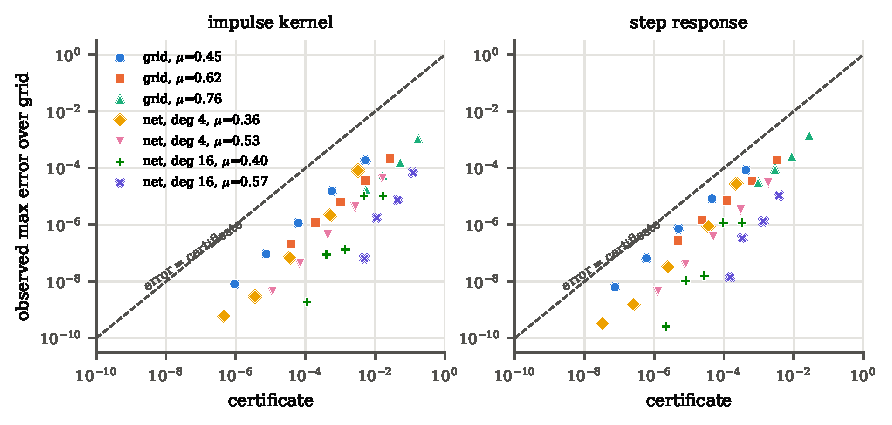
\includegraphics[width=\linewidth]{figures/fig_certificate.pdf}
\caption{Observed maximum error over the time grid against the a posteriori certificate, for the impulse kernel (left) and the step response (right), over pruning thresholds $\tau=10^{-4}$ to $10^{-12}$. Points below the dashed line are certified. Grid: $301\times301$ thermal network; net: random network with $2^{16}$ states. Reference: \texttt{expm\_multiply} on the full matrix.}\label{fig:certificate}
\end{figure}

\subsection{Memory and time versus state dimension}\label{sec:scaling}
Table~\ref{tab:scaling} and Fig.~\ref{fig:scaling} fix the query (collocated sensor and actuator, impulse kernel and step response, $\tau=10^{-10}$) and vary $N$: the thermal grid from $10^4$ to $10^{12}$ states and the degree-4 random network from $2^{16}$ to $2^{64}$. The thermal parameters are hashed from coordinates centered on the sensor, so the neighborhood of the sensor is the same at every size, and the random network is locally tree-like at every size, so the work of the walk sum should not depend on $N$. It does not. On the grid the traversal took 0.07~s and visited $1.10$ to $1.15\times10^5$ walk prefixes at every size (the small variation comes from the global bounds, which are maxima over all states), and on the network 0.02~s with $6.0$ to $7.2\times10^4$ prefixes; the peak memory of the process was 4.5 to 4.6~MB throughout. The global constants needed by the certificate were computed by a streaming pass over all states for the grid up to $10^7$ states, which took 1.1~s at $N=10^7$ and is not included in the traversal time, and from the parameter ranges otherwise.

The global methods behave as expected of state-vector methods. \texttt{expm\_multiply} on the full matrix took 0.5, 5.3, 50 and 634~s on the grid from $10^4$ to $10^7$ states and 4.6, 27, 161 and 911~s on the network from $2^{16}$ to $2^{22}$; the Arnoldi method was slower still. At $N=10^7$ its peak was 2.9~GB above the import baseline. Of this, the matrix itself accounts for 0.6~GB and most of the rest is a shifted copy of the matrix that SciPy forms internally, so a leaner implementation would need about 1~GB (the matrix and a few state vectors), still more than two orders of magnitude above the walk sum. Larger sizes were not run: at $N\ge2^{32}$ and $N\ge10^{10}$ the state vector alone exceeds the memory of the machine, and the network at $2^{24}$ was skipped for run time. All global results agreed with the walk sum to within 0.19 of its certificate. The certified ball at the walk sum's certificate has 113 states on the grid and about 1460 on the network, independent of $N$; solved by \texttt{expm\_multiply} it took 0.2 to 0.3~s and about 1~MB above the import baseline, most of the time being interpreter overhead. At these small coupling ratios both the walk sum and the ball are cheap, and the comparison that matters is the one of the next section.

\begin{table*}[t]
\footnotesize\setlength{\tabcolsep}{4pt}
\caption{Time [s] and memory [MB] versus state dimension at fixed query and pruning threshold ($\tau=10^{-10}$). Walk sum: peak memory of the C++ process. Python methods: peak minus the high-water mark after importing NumPy and SciPy (about 57~MB). Ball: certified ball at the walk sum's certificate, solved by \texttt{expm\_multiply}. n.r.: not run (state-vector methods beyond the tested range, or Krylov beyond $10^6$).}\label{tab:scaling}
\begin{ruledtabular}
\begin{tabular}{ll|cc|cc|cc|cc}
model & $N$ & \multicolumn{2}{c|}{walk sum} & \multicolumn{2}{c|}{ball + expm\_multiply} & \multicolumn{2}{c|}{expm\_multiply (full)} & \multicolumn{2}{c}{Arnoldi $m=30$ (full)}\\
 & & time [s] & mem. [MB] & time [s] & mem. [MB] & time [s] & mem. [MB] & time [s] & mem. [MB]\\\hline
thermal grid & 1.0e4 & 0.07 & 4.5 & 0.22 & 0.9 & 0.51 & 4.9 & 1.20 & 5.4 \\
thermal grid & 1.0e5 & 0.07 & 4.5 & 0.19 & 1.0 & 5.28 & 33.0 & 19 & 35.6 \\
thermal grid & 1.0e6 & 0.07 & 4.5 & 0.18 & 1.0 & 50 & 311.0 & 227 & 342.3 \\
thermal grid & 1.0e7 & 0.07 & 4.5 & 0.23 & 0.9 & 634 & 2943.6 & n.r. & n.r. \\
thermal grid & 1.0e10 & 0.07 & 4.5 & 0.26 & 1.0 & n.r. & n.r. & n.r. & n.r. \\
thermal grid & 1.0e12 & 0.07 & 4.5 & 0.31 & 0.9 & n.r. & n.r. & n.r. & n.r. \\
random net, $\Delta=4$ & $2^{16}$ & 0.02 & 4.5 & 0.30 & 1.2 & 4.59 & 21.6 & 8.65 & 23.6 \\
random net, $\Delta=4$ & $2^{18}$ & 0.02 & 4.5 & 0.28 & 1.2 & 27 & 82.6 & 39 & 88.9 \\
random net, $\Delta=4$ & $2^{20}$ & 0.03 & 4.5 & 0.29 & 1.2 & 161 & 325.5 & 243 & 357.9 \\
random net, $\Delta=4$ & $2^{22}$ & 0.02 & 4.5 & 0.29 & 1.2 & 911 & 1281.6 & n.r. & n.r. \\
random net, $\Delta=4$ & $2^{24}$ & 0.02 & 4.5 & 0.32 & 1.2 & n.r. & n.r. & n.r. & n.r. \\
random net, $\Delta=4$ & $2^{32}$ & 0.02 & 4.5 & 0.31 & 1.2 & n.r. & n.r. & n.r. & n.r. \\
random net, $\Delta=4$ & $2^{48}$ & 0.02 & 4.5 & 0.30 & 1.2 & n.r. & n.r. & n.r. & n.r. \\
random net, $\Delta=4$ & $2^{64}$ & 0.02 & 4.5 & 0.28 & 1.2 & n.r. & n.r. & n.r. & n.r. \\
\end{tabular}
\end{ruledtabular}
\end{table*}


\begin{figure}[t]
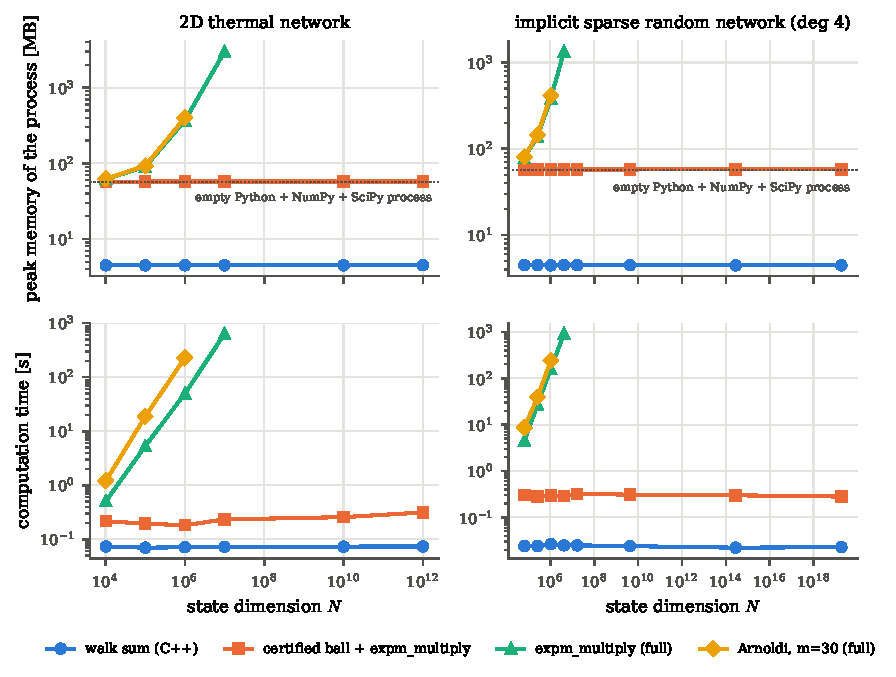
\includegraphics[width=\linewidth]{figures/fig_scaling.pdf}
\caption{Peak memory of the whole process (top) and computation time (bottom) against the state dimension, for the thermal grid ($\mu=0.45$) and the degree-4 random network ($\mu=0.36$) at fixed pruning threshold $\tau=10^{-10}$. Full-system methods were run up to $10^7$ (grid) and $2^{22}$ (network) states; larger sizes were not run. The dotted line marks the peak of a Python process that has imported NumPy and SciPy and holds no data. Data in Table~\ref{tab:scaling}.}\label{fig:scaling}
\end{figure}

\subsection{Walk sums versus certified local truncations}\label{sec:crossover}
Global methods are not the strongest competitors. A local method that propagates the state only on a set of states around the actuator has memory proportional to that set, and with the certificates of Sec.~\ref{sec:local} it carries the same guarantee as the walk sum. Table~\ref{tab:crossover} and Fig.~\ref{fig:crossover} compare the walk sum with the certified ball and the adaptive set at matched targets $10^{-3}$, $10^{-4}$ and $10^{-5}$ for the step response. The comparison covers the random network with $N=2^{64}$ at degrees 4, 16 and 32 with two values of $\mu$ each, and the thermal grid with two values of $\mu$. All three methods use the same distance information and the same compiler, and run single-threaded; the walk sum is charged the full time of its threshold search. In every case where two methods both reached the target, their outputs agreed within the sum of their certificates.

\begin{table*}[t]
\footnotesize\setlength{\tabcolsep}{1.35pt}
\caption{Walk sum versus the two certified local truncations at matched targets for the step response (forced certificate, unit input; collocated sensor and actuator, $t\le5$, $T=100$; all methods also compute the impulse kernel). Distance information is shared: Manhattan distance on the grid, a breadth-first map of radius 3 on the networks. Walk sum: certificate reached, walk prefixes visited, time of the traversal at the final threshold, cumulative time of the threshold search from the first attempt for that model (including map construction), the same cumulative time without a distance map (separate runs with a 900~s budget; ``='' where the oracle is analytic), and peak memory. Ball: radius, states, time from scratch (build, certificate, certified time integration) and peak memory. Adaptive set: states, time from scratch and peak memory. Memory is the peak of the whole process; an empty process peaks at about 4.0~MB. Rows marked $^*$ were re-timed three times on an otherwise idle machine and show medians; the spread between identical runs was up to about 40\% for sub-second walk-sum searches and a few percent for the local methods. $^\dagger$Target not reached within the 1800~s search budget (900~s without a map); best certificate shown. $^\ddagger$Not run: predicted size exceeds memory. $^\S$Stopped at the node limit without reaching the target.}\label{tab:crossover}
\begin{ruledtabular}
\begin{tabular}{lcc|cccccc|cccc|ccc}
 & & & \multicolumn{6}{c|}{walk sum} & \multicolumn{4}{c|}{certified ball} & \multicolumn{3}{c}{adaptive set}\\
graph & $\mu$ & target & cert. & prefixes & final [s] & total [s] & no map [s] & MB & $R$ & states & [s] & MB & states & [s] & MB\\\hline
net, $\Delta=4$ & 0.36 & $1\times10^{-3}$ & $3.2\times10^{-5}$ & $1.1\times10^{2}$ & $<0.01$ & $<0.01$ & $<0.01$ & 4.6 & 2 & 17 & $<0.01$ & 4.2 & 5 & $<0.01$ & 4.2 \\
net, $\Delta=4$ & 0.36 & $1\times10^{-4}$ & $3.2\times10^{-5}$ & $1.1\times10^{2}$ & $<0.01$ & $<0.01$ & $<0.01$ & 4.6 & 3 & 53 & $<0.01$ & 4.2 & 17 & $<0.01$ & 4.2 \\
net, $\Delta=4$ & 0.36 & $1\times10^{-5}$ & $6.5\times10^{-6}$ & $4.7\times10^{2}$ & $<0.01$ & $<0.01$ & $<0.01$ & 4.6 & 4 & 161 & $<0.01$ & 4.2 & 45 & $<0.01$ & 4.2 \\
net, $\Delta=4$ & 0.53 & $1\times10^{-3}$ & $3.2\times10^{-4}$ & $5.2\times10^{2}$ & $<0.01$ & $<0.01$ & $<0.01$ & 4.6 & 4 & 161 & $<0.01$ & 4.2 & 51 & $<0.01$ & 4.2 \\
net, $\Delta=4$ & 0.53 & $1\times10^{-4}$ & $8.7\times10^{-5}$ & $2.6\times10^{3}$ & $<0.01$ & $<0.01$ & 0.01 & 4.5 & 5 & 485 & $<0.01$ & 4.3 & 161 & $<0.01$ & 4.3 \\
net, $\Delta=4$ & 0.53 & $1\times10^{-5}$$^*$ & $7.7\times10^{-6}$ & $8.1\times10^{4}$ & 0.02 & 0.05 & 0.48 & 4.6 & 7 & 4373 & 0.03 & 4.7 & 1199 & $<0.01$ & 4.5 \\
net, $\Delta=16$ & 0.40 & $1\times10^{-3}$ & $6.8\times10^{-5}$ & $2.7\times10^{2}$ & $<0.01$ & $<0.01$ & $<0.01$ & 4.8 & 1 & 17 & $<0.01$ & 4.2 & 17 & $<0.01$ & 4.4 \\
net, $\Delta=16$ & 0.40 & $1\times10^{-4}$ & $6.8\times10^{-5}$ & $2.7\times10^{2}$ & $<0.01$ & $<0.01$ & $<0.01$ & 4.8 & 3 & 3857 & 0.08 & 4.6 & 257 & $<0.01$ & 4.5 \\
net, $\Delta=16$ & 0.40 & $1\times10^{-5}$$^*$ & $9.5\times10^{-6}$ & $4.8\times10^{3}$ & $<0.01$ & 0.01 & 0.93 & 4.8 & 4 & 57857 & 1.29 & 10.7 & 3857 & 0.08 & 5.0 \\
net, $\Delta=16$ & 0.57 & $1\times10^{-3}$ & $6.3\times10^{-4}$ & $2.4\times10^{3}$ & $<0.01$ & $<0.01$ & 0.04 & 4.7 & 3 & 3857 & 0.09 & 4.6 & 257 & $<0.01$ & 4.5 \\
net, $\Delta=16$ & 0.57 & $1\times10^{-4}$$^*$ & $6.1\times10^{-5}$ & $9.1\times10^{5}$ & 0.85 & 1.08 & 129 & 4.8 & 5 & $8.7\times10^{5}$ & 17 & 100.8 & 57857 & 1.39 & 14.4 \\
net, $\Delta=16$ & 0.57 & $1\times10^{-5}$ & $1.002\times10^{-5}$$^{\dagger}$ & $2.9\times10^{8}$ & -- & 1802$^{\dagger}$ & 1029$^{\dagger}$ & 4.8 & 7 & $2.0\times10^{8}$$^{\ddagger}$ & -- & -- & $2.0\times10^{7}$$^{\S}$ & -- & -- \\
net, $\Delta=32$ & 0.40 & $1\times10^{-3}$ & $2.7\times10^{-5}$ & $1.1\times10^{3}$ & $<0.01$ & $<0.01$ & $<0.01$ & 6.0 & 1 & 33 & $<0.01$ & 4.2 & 33 & $<0.01$ & 5.8 \\
net, $\Delta=32$ & 0.40 & $1\times10^{-4}$ & $2.7\times10^{-5}$ & $1.1\times10^{3}$ & $<0.01$ & 0.02 & 0.05 & 6.0 & 2 & 1025 & 0.05 & 4.3 & 806 & 0.07 & 5.8 \\
net, $\Delta=32$ & 0.40 & $1\times10^{-5}$$^*$ & $3.6\times10^{-6}$ & $3.4\times10^{4}$ & 0.09 & 0.15 & 39 & 6.0 & 3 & 31777 & 1.44 & 7.4 & 31774 & 1.51 & 10.5 \\
net, $\Delta=32$ & 0.57 & $1\times10^{-3}$ & $5.3\times10^{-4}$ & $1.1\times10^{3}$ & $<0.01$ & 0.02 & 0.06 & 6.0 & 2 & 1025 & 0.05 & 4.3 & 903 & 0.06 & 5.8 \\
net, $\Delta=32$ & 0.57 & $1\times10^{-4}$$^*$ & $6.5\times10^{-5}$ & $9.3\times10^{5}$ & 2.03 & 2.43 & 900$^{\dagger}$ & 6.0 & 5 & $3.1\times10^{7}$ & 1816 & 3028.3 & $2.7\times10^{5}$ & 13 & 53.1 \\
net, $\Delta=32$ & 0.57 & $1\times10^{-5}$ & $2.434\times10^{-5}$$^{\dagger}$ & $3.6\times10^{7}$ & -- & 1805$^{\dagger}$ & -- & 6.0 & 7 & $2.9\times10^{10}$$^{\ddagger}$ & -- & -- & $2.0\times10^{7}$$^{\S}$ & -- & -- \\
grid & 0.45 & $1\times10^{-3}$ & $1.2\times10^{-4}$ & $2.6\times10^{2}$ & $<0.01$ & $<0.01$ & = & 4.6 & 3 & 25 & $<0.01$ & 4.2 & 13 & $<0.01$ & 4.3 \\
grid & 0.45 & $1\times10^{-4}$ & $7.5\times10^{-5}$ & $4.7\times10^{2}$ & $<0.01$ & $<0.01$ & = & 4.6 & 4 & 41 & $<0.01$ & 4.2 & 21 & $<0.01$ & 4.3 \\
grid & 0.45 & $1\times10^{-5}$ & $5.6\times10^{-6}$ & $8.1\times10^{3}$ & $<0.01$ & 0.02 & = & 4.6 & 5 & 61 & $<0.01$ & 4.2 & 40 & $<0.01$ & 4.2 \\
grid & 0.62 & $1\times10^{-3}$ & $8.3\times10^{-4}$ & $3.1\times10^{3}$ & $<0.01$ & $<0.01$ & = & 4.5 & 6 & 85 & $<0.01$ & 4.2 & 25 & $<0.01$ & 4.3 \\
grid & 0.62 & $1\times10^{-4}$$^*$ & $7.0\times10^{-5}$ & $2.7\times10^{5}$ & 0.21 & 0.33 & = & 4.6 & 8 & 145 & $<0.01$ & 4.2 & 57 & $<0.01$ & 4.3 \\
grid & 0.62 & $1\times10^{-5}$$^*$ & $9.9\times10^{-6}$ & $9.9\times10^{6}$ & 6.51 & 11 & = & 4.6 & 10 & 221 & $<0.01$ & 4.2 & 81 & $<0.01$ & 4.3 \\
\end{tabular}
\end{ruledtabular}
\end{table*}


On the networks of degree 16 and 32 the walk sum was the fastest method from scratch at every target that any method certified; at degree 4 all three methods finished within 0.06~s, the adaptive set first. The walk sum's peak stayed between 4.5 and 6.1~MB. The 6.1~MB includes about 1.5~MB for the distance map at degree 32. The gap widens with the degree and with $\mu$. At degree 16 and $\mu=0.57$, target $10^{-4}$, the walk sum took 1.1~s in total (0.85~s for the final traversal) and 4.8~MB. The adaptive set took 1.4~s and 14~MB with 57\,857 states, and the ball 17~s and 101~MB with $8.7\times10^5$ states. At degree 32 and $\mu=0.57$, target $10^{-4}$, the walk sum took 2.4~s and 6.0~MB. The adaptive set took 13~s and 53~MB with $2.7\times10^5$ states, and the ball, of radius 5, took 1816~s and 3.0~GB with $3.1\times10^7$ states, of which 256~s went into building it. On the two hardest network cases, $\mu=0.57$ at target $10^{-5}$, no method certified the target. The walk sum ended its 1800~s search at $1.0015\times10^{-5}$ (degree 16) and $2.4\times10^{-5}$ (degree 32); the balls would have $2\times10^8$ and $3\times10^{10}$ states; and the adaptive set stopped at its limit of $2\times10^7$ states, after 1859 and 1054~s, with certificates of $1.5\times10^{-5}$ and $2.9\times10^{-5}$. Tiny local sets are slightly leaner than the walker: a 17-state ball peaks at 4.2~MB against the walker's 4.6~MB, because the latter carries its stack and divided-difference workspace.

On the grid the result is reversed. At $\mu=0.62$ and target $10^{-5}$ the ball needs 221 states and the adaptive set 81, and both finish in under 10~ms, while the walk sum visits $9.9\times10^6$ walk prefixes and needs 6.5~s for its final traversal and 11~s in total. Walk enumeration cannot merge walks that end at the same state, and on a lattice the number of walks of length $q$ between two states exceeds the number of states within distance $q$ by a factor that grows exponentially with $q$. On a locally tree-like graph few walks merge, so the adaptive set and the set of walk prefixes are of similar size. The walk sum then has the advantage that its temporal work is lazy, incurred only where a prefix reaches a source, while a local method integrates every retained state over the whole time grid.

A single realization can mislead, so Table~\ref{tab:ensemble} repeats the two headline cases ($\mu=0.57$, target $10^{-4}$) for three graph seeds and three actuator states each, with threshold searches started from scratch. At degree 16 the walk sum reached the target in 0.8 to 1.6~s with 4.7 to 4.8~MB. The adaptive set took 1.4 to 15~s and 14 to 99~MB, a median of 9 times longer; the realization of Table~\ref{tab:crossover} was the least favorable of the nine, at a factor of 1.5. The ball took 14 to 16~s, except for one actuator for which its certificate required radius 6, $1.3\times10^7$ states and 471~s. At degree 32 the walk sum took 2.2 to 4.0~s with 5.9 to 6.0~MB, and the adaptive set 12 to 76~s (5.5 to 19 times longer, median 8) with 53 to 173~MB. The peaks of the step responses ranged from 0.012 to 0.038. To gauge the certificates we compared each output with a reference walk sum at one hundredth of the final threshold. Lowering the threshold only enlarges the retained walk set, because the subtree bounds do not depend on it, and all contributions are positive here; the difference from the reference is therefore a lower bound on the truncation error of the coarser sum, apart from the separately assessed rounding, while the difference plus the reference's own certificate is an upper bound. The walk-sum outputs differed from the reference by $2\times10^{-7}$ to $3\times10^{-7}$ at degree 16 and by $3\times10^{-11}$ to $1.5\times10^{-8}$ at degree 32. The certificates, $6\times10^{-5}$ to $10^{-4}$, exceed these differences by factors of up to 440 and $2\times10^6$, which are thus upper bounds on their looseness. The adaptive outputs differed from the same reference by $9\times10^{-9}$ to $2\times10^{-8}$; this difference has no one-sided meaning, because the adaptive set's retained walks are not nested with those of the walk sum and it also carries a time-truncation error. These factors bound the looseness from above but do not determine it; the conservatism of the certificates is measured against independent references in Sec.~\ref{sec:accuracy}.

\begin{table*}[t]
\footnotesize\setlength{\tabcolsep}{2.4pt}
\caption{Robustness of the comparison at $\mu=0.57$, target $10^{-4}$ (step response, collocated), over three graph seeds and three actuator states ($a_1=1\,234\,567$, $a_2=987\,654\,321$, $a_3=2^{40}+12\,345$), with the radius-3 distance map. Peak: maximum of the step response. Diff.: maximum over the grid of the difference from a reference walk sum at one hundredth of the final threshold; for the walk sum it is a lower bound on its truncation error (the reference retains a superset of its walks, and all contributions are positive), for the adaptive set it is only a difference. Walk sum: certificate, difference, prefixes, total time of a threshold search started from scratch at $\varepsilon/100$, peak memory. Adaptive set: states, time, peak memory, difference. The ball was run at degree 16 only; at degree 32 one ball takes about 30~min and 3~GB (Table~\ref{tab:crossover}). n.r.: not run.}\label{tab:ensemble}
\begin{ruledtabular}
\begin{tabular}{rrrc|cccrc|crcc|crc}
 & & & & \multicolumn{5}{c|}{walk sum} & \multicolumn{4}{c|}{adaptive set} & \multicolumn{3}{c}{certified ball}\\
$\Delta$ & seed & act. & peak & cert. & diff. & prefixes & [s] & MB & states & [s] & MB & diff. & states & [s] & MB\\\hline
16 & 7 & $a_1$ & $2.4\times10^{-2}$ & $6.6\times10^{-5}$ & $2.5\times10^{-7}$ & $7.9\times10^{5}$ & 0.95 & 4.8 & 57857 & 1.39 & 14.3 & $9.2\times10^{-9}$ & $8.7\times10^{5}$ & 14 & 100.8 \\
16 & 7 & $a_2$ & $3.2\times10^{-2}$ & $7.0\times10^{-5}$ & $2.6\times10^{-7}$ & $9.5\times10^{5}$ & 0.91 & 4.8 & $3.7\times10^{5}$ & 8.47 & 64.8 & $9.0\times10^{-9}$ & $8.7\times10^{5}$ & 15 & 107.5 \\
16 & 7 & $a_3$ & $3.1\times10^{-2}$ & $7.0\times10^{-5}$ & $2.5\times10^{-7}$ & $8.9\times10^{5}$ & 0.94 & 4.8 & $3.3\times10^{5}$ & 8.20 & 55.7 & $8.9\times10^{-9}$ & $8.7\times10^{5}$ & 15 & 94.2 \\
16 & 11 & $a_1$ & $3.6\times10^{-2}$ & $7.9\times10^{-5}$ & $2.1\times10^{-7}$ & $1.1\times10^{6}$ & 1.42 & 4.8 & $5.4\times10^{5}$ & 13 & 98.9 & $1.4\times10^{-8}$ & $8.7\times10^{5}$ & 16 & 100.8 \\
16 & 11 & $a_2$ & $2.6\times10^{-2}$ & $6.9\times10^{-5}$ & $2.8\times10^{-7}$ & $1.0\times10^{6}$ & 1.16 & 4.7 & $3.9\times10^{5}$ & 9.16 & 68.1 & $1.3\times10^{-8}$ & $8.7\times10^{5}$ & 15 & 100.8 \\
16 & 11 & $a_3$ & $3.8\times10^{-2}$ & $8.3\times10^{-5}$ & $1.9\times10^{-7}$ & $1.1\times10^{6}$ & 1.59 & 4.8 & $5.8\times10^{5}$ & 15 & 98.4 & $1.4\times10^{-8}$ & $1.3\times10^{7}$ & 471 & 1274.4 \\
16 & 23 & $a_1$ & $3.3\times10^{-2}$ & $7.3\times10^{-5}$ & $2.7\times10^{-7}$ & $1.1\times10^{6}$ & 1.18 & 4.8 & $4.7\times10^{5}$ & 11 & 80.0 & $1.2\times10^{-8}$ & $8.7\times10^{5}$ & 14 & 100.8 \\
16 & 23 & $a_2$ & $2.6\times10^{-2}$ & $6.7\times10^{-5}$ & $2.4\times10^{-7}$ & $8.0\times10^{5}$ & 0.79 & 4.8 & $2.4\times10^{5}$ & 5.98 & 43.4 & $8.7\times10^{-9}$ & $8.7\times10^{5}$ & 14 & 100.8 \\
16 & 23 & $a_3$ & $3.1\times10^{-2}$ & $7.0\times10^{-5}$ & $2.5\times10^{-7}$ & $9.1\times10^{5}$ & 0.91 & 4.8 & $3.6\times10^{5}$ & 8.15 & 65.6 & $9.4\times10^{-9}$ & $8.7\times10^{5}$ & 16 & 100.8 \\
32 & 7 & $a_1$ & $1.2\times10^{-2}$ & $6.4\times10^{-5}$ & $3.9\times10^{-11}$ & $9.5\times10^{5}$ & 2.21 & 5.9 & $2.7\times10^{5}$ & 12 & 53.1 & $1.6\times10^{-8}$ & n.r. & n.r. & n.r. \\
32 & 7 & $a_2$ & $1.6\times10^{-2}$ & $7.3\times10^{-5}$ & $5.6\times10^{-10}$ & $1.1\times10^{6}$ & 2.43 & 5.9 & $4.9\times10^{5}$ & 22 & 79.3 & $1.6\times10^{-8}$ & n.r. & n.r. & n.r. \\
32 & 7 & $a_3$ & $1.6\times10^{-2}$ & $7.0\times10^{-5}$ & $6.9\times10^{-10}$ & $1.1\times10^{6}$ & 2.48 & 5.9 & $4.4\times10^{5}$ & 20 & 74.4 & $1.6\times10^{-8}$ & n.r. & n.r. & n.r. \\
32 & 11 & $a_1$ & $1.8\times10^{-2}$ & $9.2\times10^{-5}$ & $1.3\times10^{-8}$ & $1.1\times10^{6}$ & 3.83 & 6.0 & $9.9\times10^{5}$ & 68 & 173.1 & $1.3\times10^{-8}$ & n.r. & n.r. & n.r. \\
32 & 11 & $a_2$ & $1.3\times10^{-2}$ & $7.5\times10^{-5}$ & $2.8\times10^{-9}$ & $1.1\times10^{6}$ & 3.22 & 6.0 & $5.1\times10^{5}$ & 26 & 80.2 & $2.0\times10^{-8}$ & n.r. & n.r. & n.r. \\
32 & 11 & $a_3$ & $1.9\times10^{-2}$ & $9.8\times10^{-5}$ & $1.5\times10^{-8}$ & $1.1\times10^{6}$ & 4.04 & 6.0 & $9.9\times10^{5}$ & 76 & 168.2 & $1.1\times10^{-8}$ & n.r. & n.r. & n.r. \\
32 & 23 & $a_1$ & $1.6\times10^{-2}$ & $8.2\times10^{-5}$ & $5.7\times10^{-9}$ & $1.1\times10^{6}$ & 3.27 & 6.0 & $6.2\times10^{5}$ & 32 & 108.1 & $1.6\times10^{-8}$ & n.r. & n.r. & n.r. \\
32 & 23 & $a_2$ & $1.3\times10^{-2}$ & $6.5\times10^{-5}$ & $3.3\times10^{-11}$ & $1.0\times10^{6}$ & 2.38 & 5.9 & $3.1\times10^{5}$ & 14 & 56.8 & $1.5\times10^{-8}$ & n.r. & n.r. & n.r. \\
32 & 23 & $a_3$ & $1.5\times10^{-2}$ & $7.2\times10^{-5}$ & $7.7\times10^{-10}$ & $1.1\times10^{6}$ & 2.88 & 6.0 & $4.8\times10^{5}$ & 23 & 79.6 & $1.7\times10^{-8}$ & n.r. & n.r. & n.r. \\
\end{tabular}
\end{ruledtabular}
\end{table*}


Distance information matters as much as the method. Without the distance map, which is the walk sum's leanest configuration and the one used in Sec.~\ref{sec:scaling}, the same searches took 129~s instead of 1.1~s at degree 16 and $\mu=0.57$, target $10^{-4}$, and 39~s instead of 0.15~s at degree 32 and $\mu=0.40$, target $10^{-5}$ (the runs without a map are single measurements from a separate session). At degree 32 and $\mu=0.57$, target $10^{-4}$, the search did not reach the target within 900~s; a separate run at a supplied threshold needed 1333~s. A map of radius $r_d$ stores as many states as a ball of radius $r_d$, so the radius is a memory-for-time knob. At $r_d=3$ it added at most about 1.5~MB to the process here, and it is the reason the walk sum wins on these graphs.


\begin{figure*}[t]
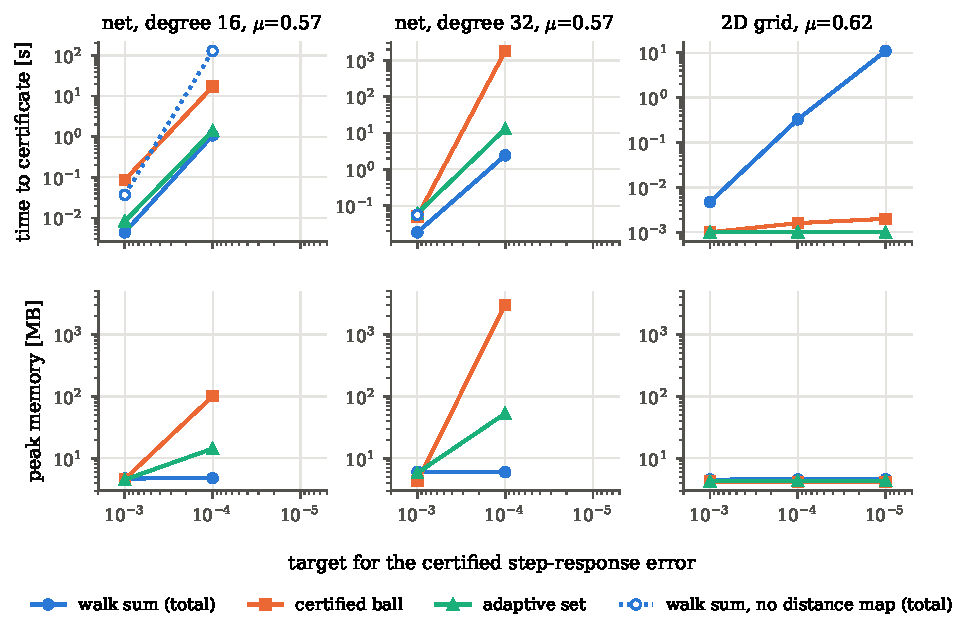
\includegraphics[width=0.85\textwidth]{figures/fig_crossover_v2.pdf}
\caption{Time to a certified step-response error from scratch (top) and peak memory of the process (bottom) for three of the graphs of Table~\ref{tab:crossover}. Walk sum: cumulative time of the threshold search, with the shared distance information (solid) and without a distance map (dotted, time only). Targets not reached by a method are omitted; on the two networks no method reached $10^{-5}$. Times below $10^{-3}$~s are plotted at $10^{-3}$~s; re-timed rows of Table~\ref{tab:crossover} enter as medians.}\label{fig:crossover}
\end{figure*}

\subsection{Separated actuator and sensor}\label{sec:noncol}
The comparisons so far use a collocated sensor, a return response. A transfer response between distinct states is smaller, and a certificate is useful only if it is small compared with the response, since the certificate is absolute (Sec.~\ref{sec:batch}). Table~\ref{tab:noncol} therefore sets the target to 10\% and 1\% of the peak of the step response. It places the sensor 2 and 4 hops from the actuator on the degree-4 network, 1 and 2 hops away on the degree-16 network, and 2 and 4 sites away on the grid. The networks use a radius-4 distance map, so that the sensor lies inside it. The peaks range from $2.8\times10^{-4}$ (two hops, degree 4) and $3.6\times10^{-4}$ (one hop, degree 16) down to $6.4\times10^{-6}$ (two hops, degree 16) and $9.7\times10^{-7}$ (four hops, degree 4).

On the degree-16 network the walk sum kept its runtime advantage. On that network with the sensor one hop away, at 1\% of the peak, the walk sum took 0.05~s, the adaptive set 0.15~s and the ball 25~s with $8.7\times10^5$ states. Two hops away, at 10\% of a peak of $6.4\times10^{-6}$, the walk sum took 0.18~s and 7.1~MB, the adaptive set 1.8~s and 16~MB with 56\,224 states, and the ball 676~s and 1.3~GB with $1.3\times10^7$ states; the 1\% target was not attempted there. On the degree-4 network the walk sum and the adaptive set both finished within 0.02~s at every separation, too fast to rank, and the adaptive set used slightly less memory; the ball needed up to 0.4~s, because a ball that must reach a distant sensor is large in every direction. On the grid the local methods again finished in under 10~ms, while the walk sum needed 0.7~s at four sites and 1\% of the peak. The distance map accounts for the higher memory of the walk sum on the degree-16 network (7.2~MB, of which about 3~MB is the radius-4 map). In every case the three outputs agreed within the sum of their certificates.

\begin{table*}[t]
\footnotesize\setlength{\tabcolsep}{2.6pt}
\caption{Separated actuator and sensor: step response at a sensor $d$ hops from the actuator, certified to 10\% and 1\% of its peak (the peak was estimated by adaptive runs with a certificate below 3\% of it). Distance information: breadth-first map of radius 4 on the networks, Manhattan distance on the grid. Walk sum: certificate, walk prefixes, cumulative time of the threshold search from scratch, peak memory. Ball (around the actuator, containing the sensor) and adaptive set: states, time from scratch and peak memory. $^\dagger$Target not reached within 1800~s. $^\S$Adaptive set stopped at its node limit without reaching the target.}\label{tab:noncol}
\begin{ruledtabular}
\begin{tabular}{lcccc|cccc|cccc|ccc}
 & & & & & \multicolumn{4}{c|}{walk sum} & \multicolumn{4}{c|}{certified ball} & \multicolumn{3}{c}{adaptive set}\\
graph & $\mu$ & $d$ & peak & target & cert. & prefixes & [s] & MB & $R$ & states & [s] & MB & states & [s] & MB\\\hline
net, $\Delta=4$ & 0.36 & 2 & $2.8\times10^{-4}$ & 10\% & $2.9\times10^{-6}$ & $3.0\times10^{2}$ & $<0.01$ & 4.4 & 4 & 161 & $<0.01$ & 4.1 & 20 & $<0.01$ & 4.1 \\
net, $\Delta=4$ & 0.36 & 2 & $2.8\times10^{-4}$ & 1\% & $1.3\times10^{-6}$ & $5.5\times10^{2}$ & $<0.01$ & 4.5 & 5 & 485 & $<0.01$ & 4.2 & 59 & $<0.01$ & 4.2 \\
net, $\Delta=4$ & 0.36 & 4 & $9.7\times10^{-7}$ & 10\% & $4.0\times10^{-8}$ & $5.7\times10^{3}$ & $<0.01$ & 4.4 & 8 & 13121 & 0.11 & 5.6 & 494 & $<0.01$ & 4.3 \\
net, $\Delta=4$ & 0.36 & 4 & $9.7\times10^{-7}$ & 1\% & $8.5\times10^{-9}$ & $2.4\times10^{4}$ & 0.01 & 4.5 & 9 & 39365 & 0.39 & 8.5 & 1452 & 0.02 & 4.4 \\
net, $\Delta=16$ & 0.40 & 1 & $3.6\times10^{-4}$ & 10\% & $1.6\times10^{-5}$ & $1.4\times10^{3}$ & $<0.01$ & 7.2 & 4 & 57857 & 1.14 & 10.6 & 257 & 0.01 & 7.0 \\
net, $\Delta=16$ & 0.40 & 1 & $3.6\times10^{-4}$ & 1\% & $3.0\times10^{-6}$ & $1.2\times10^{4}$ & 0.05 & 7.2 & 5 & $8.7\times10^{5}$ & 25 & 100.7 & 3857 & 0.15 & 7.2 \\
net, $\Delta=16$ & 0.40 & 2 & $6.4\times10^{-6}$ & 10\% & $6.1\times10^{-7}$ & $8.3\times10^{4}$ & 0.18 & 7.1 & 6 & $1.3\times10^{7}$ & 676 & 1274.4 & 56224 & 1.84 & 16.1 \\
grid & 0.45 & 2 & $5.6\times10^{-4}$ & 10\% & $2.6\times10^{-5}$ & $1.1\times10^{3}$ & $<0.01$ & 4.5 & 5 & 61 & $<0.01$ & 4.2 & 20 & $<0.01$ & 4.1 \\
grid & 0.45 & 2 & $5.6\times10^{-4}$ & 1\% & $5.3\times10^{-6}$ & $7.4\times10^{3}$ & $<0.01$ & 4.5 & 7 & 113 & $<0.01$ & 4.1 & 44 & $<0.01$ & 4.3 \\
grid & 0.45 & 4 & $4.3\times10^{-6}$ & 10\% & $3.9\times10^{-7}$ & $4.3\times10^{4}$ & 0.02 & 4.4 & 9 & 181 & $<0.01$ & 4.2 & 56 & $<0.01$ & 4.2 \\
grid & 0.45 & 4 & $4.3\times10^{-6}$ & 1\% & $3.1\times10^{-8}$ & $9.9\times10^{5}$ & 0.72 & 4.5 & 11 & 265 & $<0.01$ & 4.2 & 75 & $<0.01$ & 4.2 \\
\end{tabular}
\end{ruledtabular}
\end{table*}



\subsection{Stiffness}\label{sec:stiff}
Exact integration of the diagonal makes the cost of the walk sum depend only weakly on stiffness that resides in the diagonal. To test this we drew the thermal capacities of the $317\times317$ grid log-uniformly over $s_C$ decades below one; the comparison ratios, and with them the walk structure, do not depend on the capacities, while $\|A\|_1$ grows from 26 ($s_C=0$) to 193, 1921 and 19\,157 ($s_C=1,2,3$). Table~\ref{tab:stiff} lists the results. The walk sum visited the same 112\,429 walk prefixes at every $s_C$ and took 0.08 to 0.16~s; the increase comes from the squaring levels of the divided-difference kernel, which grew from 2 to 11. Full-system \texttt{expm\_multiply}, whose cost grows with $\|A\|t$, took 5.4, 6.4, 92 and 236~s, and the implicit BDF integrator, nearly insensitive to stiffness but slow at the tolerance needed to match ($10^{-10}$ relative), 123 to 150~s.

The local methods need only a few states here: the certified ball 113 and the adaptive set 57, at the walk sum's certificate. With the compiled explicit Taylor integrator their cost grows with $\|A\|$. The ball took 0.001, 0.006, 0.07 and 0.67~s for $s_C=0$ to 3, and the adaptive set 0.005, 0.008, 0.04 and 0.33~s, so the local methods are faster for $s_C\le2$ and the walk sum is faster at $s_C=3$. Solved with SciPy's BDF integrator, the ball took 0.3 to 0.5~s at every $s_C$, most of it interpreter overhead. A compiled implicit integrator on the ball would presumably remove the stiffness dependence of the local methods as well; we did not implement one. All methods agreed with the walk sum within its certificate.

\begin{table}[t]
\footnotesize\setlength{\tabcolsep}{1.8pt}
\caption{Stiffness sweep on the $317\times317$ thermal grid (capacities log-uniform over $s_C$ decades; step response, $t\le5$, $N=1.0\times10^5$). $\|A\|_1$ is the bound reported by the walker. Times in s; walk-sum memory is the process peak in MB. Full grid: SciPy \texttt{expm\_multiply} (Taylor) and variable-order BDF. Certified ball (113 states): compiled Taylor integrator with certified time truncation, and SciPy BDF. Adaptive set (57 states): compiled Taylor integrator. Local methods are certified at the walk sum's certificate.}\label{tab:stiff}
\begin{ruledtabular}
\begin{tabular}{rr|rrr|rr|rr|r}
 & & \multicolumn{3}{c|}{walk sum} & \multicolumn{2}{c|}{full grid} & \multicolumn{2}{c|}{ball} & adapt.\\
$s_C$ & $\|A\|_1$ & prefixes & time & mem. & Taylor & BDF & Taylor & BDF & Taylor\\\hline
0 & 26 & 112429 & 0.10 & 4.5 & 5.43 & 123 & $<0.01$ & 0.31 & $<0.01$ \\
1 & 193 & 112429 & 0.07 & 4.6 & 6.37 & 132 & $<0.01$ & 0.49 & $<0.01$ \\
2 & 1921 & 112429 & 0.08 & 5.0 & 92 & 144 & 0.07 & 0.37 & 0.04 \\
3 & 19157 & 112429 & 0.16 & 4.4 & 236 & 150 & 0.67 & 0.40 & 0.33 \\
\end{tabular}
\end{ruledtabular}
\end{table}


\subsection{Batches of times and inputs, and the number of sensors and actuators}\label{sec:batch}
On the random network with $2^{40}$ states ($\mu=0.36$, $\tau=10^{-10}$, horizon $t\le5$), increasing the number of output samples from $T=10$ to $T=1000$ changed the traversal time from 6.2 to 12.9~ms and the divided-difference workspace from 3.7 to 81~kB; the number of visited prefixes (18\,824) and of temporal row computations (1230) is independent of $T$, because the temporal work is lazy and the enumeration dominates. Adding input patterns is similarly cheap while the arithmetic stays real: one, two and four patterns (step, ramp, quadratic, decaying exponential) took 5.3, 6.3 and 7.6~ms. Including a cosine forces complex arithmetic and, with eight patterns, took 79~ms.

Reuse across input waveforms follows from Sec.~\ref{sec:piecewise}. On a network with $2^{18}$ states, one traversal produced the step kernel in 0.049~s (certificate $1.3\times10^{-7}$ per unit input), after which 100 zero-order-hold waveforms with 20 random levels each were evaluated by discrete convolution in 0.013~s in total. Propagating the full state through the same waveforms with \texttt{expm\_multiply} took 47~s per waveform (three waveforms run), and agreed with the convolution to $4.4\times10^{-9}$. The kernel route is available to any method that can produce a step response once; what the walk formulation adds is that the step, ramp and higher kernels come from the same traversal.

On the thermal grid ($\mu=0.45$, $\tau=10^{-10}$, with the Manhattan distance oracle), the traversal time grew linearly with the number of sensors (0.035, 0.049, 0.085, 0.20, 0.35~s for $p=1,2,4,8,16$ adjacent sensors, each a separate root) and sublinearly with the number of actuators (0.034 to 0.22~s for $m=1$ to 16, sharing traversals). Separating sensor and actuator by $d$ hops reduces the response by an order of magnitude or more per hop (from $7.0\times10^{-2}$ at $d=0$ to $8.9\times10^{-11}$ at $d=8$) while the certificate at fixed $\tau$ stays near $10^{-6}$, so from $d\approx4$ on the certificate exceeds the response: certificates are absolute, and a small separated response needs a proportionally smaller threshold. The distance oracle reduced the number of visited prefixes by a factor of 2.4 at $d=0$ and 29 at $d=8$.

\subsection{Unfavorable regimes}\label{sec:hard}
\begin{figure}[t]
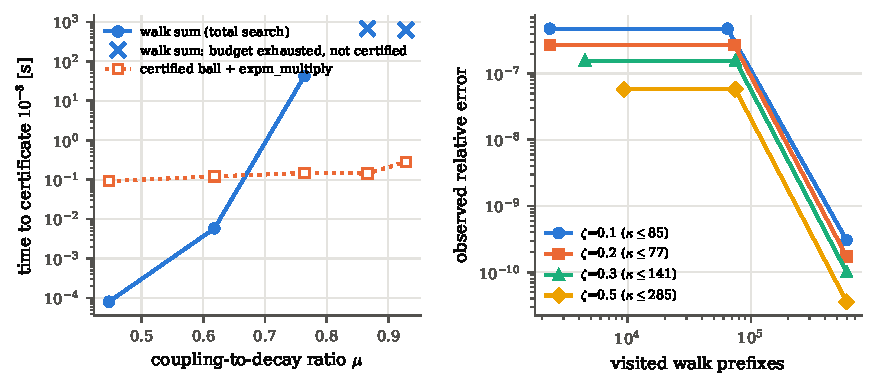
\includegraphics[width=\linewidth]{figures/fig_hard.pdf}
\caption{Unfavorable regimes. Left: time to reach a certificate of $10^{-3}$ on the step response of the $317\times317$ thermal grid as the coupling-to-decay ratio $\mu$ approaches one; for the walk sum the total time of the threshold search, with crosses where the search stopped without a certificate (plotted at the time spent; the next attempt would have exceeded the 900~s budget). Right: oscillator network in local modal coordinates; observed error relative to the response against the number of visited walk prefixes, for four damping ratios; $\kappa$ is the largest cancellation indicator over the time grid.}\label{fig:hard}
\end{figure}

\paragraph*{Coupling-to-decay ratio near one.} On the $317\times317$ thermal grid we lowered the convective loss until $\mu$ approached one and asked both methods for a certificate of $10^{-3}$ on the step response (Fig.~\ref{fig:hard}, left). The walk sum needed $8\times10^{-5}$~s at $\mu=0.45$, $6\times10^{-3}$~s at $\mu=0.62$ and 42~s at $\mu=0.76$ (total search time). At $\mu=0.87$ and $\mu=0.93$ it did not reach the target within the 900~s budget; the best certificates were $3.1\times10^{-2}$ and $0.41$, after visiting about $10^8$ and $5\times10^7$ prefixes in the last attempt. The certified ball needed radii 2 to 43 and at most 3785 states, and took 0.1 to 0.3~s in SciPy at every $\mu$. On a lattice this is the expected outcome: the ball grows polynomially with the radius while the walk count grows exponentially with the depth.

\paragraph*{Oscillatory dynamics and cancellation.} A $31\times31$ network of unit masses on grounding springs with dampers (damping ratio $\zeta$) and weak neighbor springs ($\kappa=0.05$) is a stable second-order system whose scalar diagonal splitting would place the local oscillation into the couplings. We therefore transformed each unit to its local modal coordinates, a $2\times2$ change of basis per unit, which leaves complex conjugate diagonal entries $-\zeta\omega\pm i\omega\sqrt{1-\zeta^2}$ and complex couplings ($N=1922$). The walk sum of the velocity response to a force at the same unit, computed in complex arithmetic, reproduced the real physical kernel with imaginary parts below $2\times10^{-16}$. For $\zeta=0.5$ and $0.3$ the uniform certificate applies ($\mu=0.46$, $0.70$); for $\zeta=0.2$ and $0.1$, $\mu=1.02$ and $2.0$ and only the finite-horizon certificate is available, which on $t\le5$ still certified $7\times10^{-6}$ and $1\times10^{-5}$ at $\tau=10^{-10}$ (observed errors $1.7\times10^{-10}$ and $3.0\times10^{-10}$ relative to a response of order one). The cost was the same at all four damping ratios, about $6\times10^5$ visited prefixes and 0.7~s, because over this short horizon the bounds are dominated by the couplings. The cancellation indicator, however, was 77 to 285: contributions of opposite phase cancel, and rounding errors are amplified by that factor; at the smallest threshold the observed errors were still dominated by truncation. For longer horizons the finite-horizon bound grows like $e^{\beta t}$, so for lightly damped oscillators observed over many periods we expect the cost to rise quickly; we did not test such horizons.

\paragraph*{Directed transport.} On an upwind advection chain with weak back-diffusion, $\dot x_i=-(a+\ell_i+\epsilon)x_i+a\,x_{i-1}+\epsilon\,x_{i+1}$ ($a=5$, $N=4000$), the walk sum is exact and essentially free without back-diffusion (27 prefixes visited, error $3\times10^{-16}$), because only one walk connects the actuator to a downstream sensor. Back-diffusion introduces excursions: with $\epsilon=0.2$, a sensor 20 sites downstream cost $2.4\times10^7$ visited prefixes and 34~s (certificate $6.7\times10^{-7}$, observed error $3.9\times10^{-8}$), and with $\epsilon=1$ the collocated response alone cost $6.8\times10^8$ visited prefixes and 110~s, against 0.2~s for \texttt{expm\_multiply} on the whole chain. For sensors 10 and 20 sites downstream at $\epsilon=1$ the traversal reached its 600~s limit (about $10^9$ and $2.5\times10^8$ prefixes) without a valid certificate; the partial sums were off by 11\% and 59\% of the response.

\paragraph*{Transient growth.} A regime in which only the finite-horizon bound applies is a directed chain with strong forward coupling, $\dot x_i=-(h_i+\epsilon)x_i+a\,x_{i-1}+\epsilon\,x_{i+1}$ with $a=3$, $h_i\in[0.75,1.25]$ and $N=2000$, for which $\mu$ is between 3 and 4 and $\max_{t\le5}\|e^{tA}\|_2\approx3\times10^4$ (computed on the leading 300 states). Without back-coupling ($\epsilon=0$) the chain is stable, with spectral abscissa $-0.75$, but strongly nonnormal; the walk sum is exact, with 22 prefixes visited, and the observed differences from \texttt{expm\_multiply} were at the level of rounding relative to the response ($8\times10^{-15}$ relative for a sensor ten sites downstream, where the response reaches 892). With $\epsilon=0.1$ the chain is weakly unstable (abscissa $+0.12$, from the symmetrized tridiagonal form). The collocated response was certified to $2.1\times10^{-8}$ after $8.3\times10^7$ visited prefixes in 58~s, and the response five sites downstream to $6.8\times10^{-8}$ after $2.0\times10^8$ prefixes in 302~s (observed errors $3\times10^{-11}$ and $5\times10^{-10}$); ten sites downstream the traversal reached its 600~s limit. With $\epsilon=0.3$ (abscissa $+0.70$) none of the three sensor positions was certified within 600~s, and the partial sums were off by 73 to 88\% of the response. \texttt{expm\_multiply} on the whole chain took 0.15 to 0.20~s in every case. When $\beta t$ is large and the couplings allow back-and-forth excursions, the walk sum is not a competitive method.

\section{Discussion}\label{sec:discussion}

The memory accounting of Sec.~\ref{sec:algorithm} holds in practice. With an implicit model and no distance map, the working set is the path stack, the in-edge buffers, the divided-difference workspace and the output accumulators, a few kilobytes on top of a 4~MB process, and it does not change between $N=10^4$ and $N=2^{64}$. The state vector is never formed, and neither is a Krylov basis. Three things are still stored and should not be forgotten: an explicit model, when the model is explicit; the distance map, when one is used, which holds the states of a ball of radius $r_d$ and cost up to about 1.5~MB at $r_d=3$ and 3~MB at $r_d=4$ here; and the outputs, which scale with the number of sensors, inputs, patterns and time samples. The memory figures quoted in this paper include all three.

Whether the method is useful is decided by the number of walk prefixes that have to be visited to reach a certificate, and that number depends on four things. The first is the comparison ratio $\mu$, which sets how fast the contribution of long walks decays. The cost grows steeply as $\mu$ approaches one, and for $\mu\ge1$ only the finite-horizon bound is available, with a depth that grows with $\beta t$. On the directed chains of Sec.~\ref{sec:hard}, where back-coupling creates many excursions, the walk sum was slower than \texttt{expm\_multiply} on the whole chain by two to three orders of magnitude or did not certify at all. The second is the in-degree, which sets the branching. The third is the distance information available to the bounds: on the networks a radius-3 map reduced the time to a certificate by factors of about 10 to several hundred, for at most about 1.5~MB. The fourth, which decides the comparison with local methods, is how often distinct walks end at the same state. A local state vector merges all walks that reach a state; walk enumeration cannot, because the temporal factor of a walk depends on its whole multiset of diagonal entries. On a lattice this costs the walk sum orders of magnitude. On a locally tree-like graph few walks merge, the set of visited prefixes and the adaptive set are of similar size, and the walk sum then gains from doing temporal work only where a prefix reaches a source. A local method, in contrast, integrates every retained state over the whole time grid. The uniform ball is the weakest of the three on such graphs because its size is set by its radius, $(\Delta-1)^R$, rather than by the weights. The runtime advantage over the adaptive set also held in the tested degree-16 transfer responses between separated states; the degree-4 cases were too fast to rank reliably (Sec.~\ref{sec:noncol}).

The memory comparison is less one-sided than the extreme cases suggest. The walk sum's memory stays nearly fixed, between 4.5 and 6.1~MB here including the distance map, while the local methods' memory grows with their sets; tiny local sets are in fact slightly leaner than the walker, and the large savings (a factor of 9 against the adaptive set and of about 500 against the ball at degree 32, $\mu=0.57$, target $10^{-4}$, and 3 to 29 against the adaptive set over the realizations of Table~\ref{tab:ensemble}) appear only once the retained sets reach $10^5$ to $10^7$ states.

Several limitations are worth stating plainly. The certificates are worst-case over the endpoints of the discarded walks. Against \texttt{expm\_multiply} references (Fig.~\ref{fig:certificate}; no distance map on the networks) they were loose by one to two orders of magnitude on the lattice and by up to four on the tree-like networks, where a discarded walk rarely returns to the sensor but is charged as if it did. The comparisons with tighter walk sums in Table~\ref{tab:ensemble} provide upper bounds on certificate looseness, up to $2\times10^6$ at degree 32, but do not determine its magnitude. Because the cost grows faster than the inverse certificate, tighter bounds would translate directly into lower cost, and the largest gain is to be had on exactly the graphs where the walk sum is competitive. Any improved completion bound applies equally to the adaptive set, whose certificate (Proposition~\ref{prop:local}) uses the same completion estimate, so whether it would favor walk enumeration is an open question. The distance oracle already enters the certificate, through the factor $\mu^{\delta_k}$ for the shortest completion, but beyond that the bound lets every step of a completion head back toward the sources. Bounds that use how few completions actually return, for instance through return probabilities on locally tree-like graphs, are the natural next step. The uniform-in-time bound needs $\mu<1$; diagonal scaling can extend it, but an optimized scaling vector is itself a state-sized object. Oscillatory systems produce cancellation between walks, which we monitor but do not remove. The scalar diagonal splitting integrates only scalar local dynamics exactly; second-order units were handled here by a local modal transformation, and a genuine block-diagonal splitting would require divided differences of matrix arguments. Finally, the method computes responses at prescribed times; it does not by itself provide controllability measures, reduced models or closed-loop behavior.

Two extensions are immediate from the formulas but were not developed here. Parametric sensitivities come almost for free: a walk visiting state $i$ $m_i$ times satisfies $\partial_{d_i}f_t[\mathcal{D}_p]=m_if_t[\mathcal{D}_p,d_i]$, so the derivative of an output with respect to a local decay rate is one more appended node (verified numerically in Appendix~\ref{app:verification}). And memoization interpolates between walks and state vectors: storing the forward response at the states of a small ball around the actuator and enumerating walks from the sensor only until they reach that ball would trade memory for time continuously, at the price of a convolution on the time grid that the present exact scheme avoids.


\begin{acknowledgments}
We acknowledge support from ARL. [Award details to be supplied by the authors.]
\end{acknowledgments}

\appendix
\section{Time-dependent generators}\label{app:td}

The walk representation extends to $\dot\bx=A(t)\bx+\bb(t)$ when the time dependence is a sum of exponentials, through the integral-free Dyson series of Ref.~\cite{kalev2021}. We record the resulting formulas and their numerical checks; they are not used elsewhere in the paper.

Let $A(t)=E+V(t)$ with $E=\mathrm{diag}(E_1,\dots,E_N)$ constant and
\begin{equation}
V(t)=\sum_{i}\sum_{k}e^{\lambda_{ik}t}D_{ik}P_i ,
\end{equation}
where each $P_i$ is a permutation, $D_{ik}$ is diagonal, and $P_0=I$ is included, so that time-dependent diagonal terms are events too. Neither $E$ nor $V$ needs to be diagonalizable; $E$ is simply the diagonal in the coordinate basis. With the interaction picture
\begin{equation}
\Phi(t,0)=e^{Et}\Phi_I(t),\qquad \dot\Phi_I(t)=e^{-Et}V(t)e^{Et}\Phi_I(t),
\end{equation}
an event sequence that visits states $u_0,u_1,\dots,u_q$ through terms $(i_r,k_r)$ has amplitude $d_r=(D_{i_rk_r})_{u_ru_r}$, evaluated at the destination $u_r$, and rate $\lambda_r=\lambda_{i_rk_r}$. The number of events $q$ counts both genuine hops ($i_r\neq0$) and diagonal events ($i_r=0$), so it can exceed the number of off-diagonal hops.

\begin{proposition}
The contribution of the sequence to $\Phi(t,s)\be_{u_0}$ is $\be_{u_q}$ times
\begin{equation}\label{eq:td_path}
\begin{gathered}
\Big(\prod_{r=1}^qd_r\Big)\,e^{s\Lambda_p}\,f_{t-s}[y_0,\dots,y_q],\\
y_j=E_{u_j}+\sum_{r=j+1}^q\lambda_r,\qquad \Lambda_p=\sum_{r=1}^q\lambda_r .
\end{gathered}
\end{equation}
Consequently a forcing $\bb(t)=\be_{u_0}e^{\gamma t}$ contributes $\big(\prod_rd_r\big)f_t[y_0,\dots,y_q,\gamma+\Lambda_p]$ to $\int_0^t\Phi(t,s)\bb(s)ds$.
\end{proposition}
\begin{proof}
Take $s=0$ first. The contribution obeys $c_q(t)=\int_0^te^{E_{u_q}(t-\sigma)}d_qe^{\lambda_q\sigma}c_{q-1}(\sigma)d\sigma$ with $c_0(t)=e^{E_{u_0}t}$. Suppose $c_{q-1}(\sigma)=\prod_{r<q}d_r\,f_\sigma[y'_0,\dots,y'_{q-1}]$ with $y'_j=E_{u_j}+\sum_{j<r<q}\lambda_r$. By (D3), $e^{\lambda_q\sigma}f_\sigma[y']=f_\sigma[y'+\lambda_q]$, and $y'_j+\lambda_q=y_j$. Proposition~\ref{prop:forcing} with $m=0$ then gives $c_q(t)=\prod_rd_r\,f_t[y_0,\dots,y_{q-1},E_{u_q}]$, and $y_q=E_{u_q}$. For a start time $s$, write the event times as $s+\tau_r$; each factor $e^{\lambda_r(s+\tau_r)}$ releases $e^{\lambda_rs}$, and the remaining integral is $c_q(t-s)$. The forcing statement follows from Proposition~\ref{prop:forcing} applied to $\int_0^te^{s\Lambda_p}f_{t-s}[y]e^{\gamma s}ds$.
\end{proof}
The factor $e^{s\Lambda_p}$ makes $\Phi(t,s)$ depend on $s$ and not only on $t-s$, and it shifts the node appended for an exponential forcing from $\gamma$ to $\gamma+\Lambda_p$. The signs matter: the interaction picture must be taken as written above, so that the rate shifts enter the nodes with a positive sign, and diagonal events ($i_r=0$) must be included.

The regression case $A(t)=e^t\left(\begin{smallmatrix}0&1\\1&0\end{smallmatrix}\right)$, $\bx_0=(1,1)^\top$, has the exact solution $\bx(t)=\exp(e^t-1)\bx_0$. Equation~\eqref{eq:td_path} gives nodes $(q,q-1,\dots,0)$ for the $q$-event sequences and $\sum_qf_t[0,1,\dots,q]=\sum_q(e^t-1)^q/q!$, which reproduces it; reversing the signs of the rate shifts would give nodes $(-q,\dots,0)$ and $\exp(1-e^{-t})$ instead (at $t=1$, $1.8816$ instead of $5.5749$). We also checked, against a high-accuracy ODE solution, a three-state example with noncommuting $A(t)$ at different times, a cyclic permutation with two rates and a diagonal event term, start time $s=0.35$, and exponential forcing: the walk sums agree to $2\times10^{-12}$, satisfy the cocycle property $\Phi(t,s)\Phi(s,r)=\Phi(t,r)$ to $7\times10^{-12}$, and the forced response with the appended node $\gamma+\Lambda_p$ agrees to $7\times10^{-13}$, while the unshifted node $\gamma$ is off by $4\times10^{-2}$ (script \texttt{verify\_formulas.py}).

\section{Verification}\label{app:verification}

Two independent layers of checks accompany the code. The first (\texttt{verify\_formulas.py}, 38 checks) tests the formulas themselves with a slow reference implementation: divided differences against 60-digit evaluations of the Opitz exponential (relative error $\le4\times10^{-16}$ for distinct, repeated, nearly coincident at $10^{-9}$, and complex nodes); the walk expansion and the orientation of hop coefficients against dense exponentials; Proposition~\ref{prop:forcing} by adaptive quadrature, including exactly resonant rates and $m=2,3$; responses to steps, exponentials, ramps and cosines against augmented exponentials; delayed pulses and piecewise-linear inputs through the truncated-power basis against quadrature; the sensitivity identity $\partial_{d_i}f_t[\mathcal{D}]=m_if_t[\mathcal{D},d_i]$ by finite differences; and the time-dependent statements of Appendix~\ref{app:td}.

The second layer (\texttt{tests/test\_walker.py}, 32 tests, and \texttt{tests/test\_local\_solvers.py}, 14 tests) runs the C++ walker against dense references (SciPy \texttt{expm} of the system or of the augmented system, or exact propagation across breakpoints) and asserts, for every output on the grid, that the observed error lies below the a posteriori certificate plus a rounding allowance of $10^{-12}$ times the output scale; tests with exact or near-exact walk sets also assert a relative error below $10^{-11}$. The local-solver tests check the adaptive certificate of Proposition~\ref{prop:local} on sign-indefinite random networks with collocated and separated sensors, the certified time truncation of the local Taylor integrator (including decay rates spread over three decades), that the restricted generator keeps the original diagonal, and that balls built on the undirected graph certify directed cycles, for which balls of directed reachability would not. Table~\ref{tab:tests} lists what the walker tests cover. A third script, \texttt{tests/kernel\_long\_grid.py}, measures the rounding of the temporal kernel over $10^2$ to $10^5$ output samples (Sec.~\ref{sec:accuracy}).

\begin{table}[h]
\caption{Coverage of the walker test suite. Each line is one or more tests; all pass.}\label{tab:tests}
\begin{ruledtabular}
\footnotesize
\begin{tabular}{p{0.36\linewidth}p{0.56\linewidth}}
case & checks\\\hline
pure diagonal $A$ & exact local responses, no hop is taken\\
$A=0$ & step, ramp and $s^2/2$ normalization ($t$, $t^2/2$, $t^3/6$)\\
two states, distinct diagonal & kernel, step, ramp\\
repeated diagonal, resonant forcing & appended node equal to a diagonal entry, twice repeated\\
nearly coincident complex nodes & spacing $10^{-9}$; conjugate-pair cosine, imaginary residue $\le10^{-13}$\\
Jordan block & $e^{-\lambda t}t^{n-1}/(n-1)!$, finite walk set\\
directed cycle & repeated visits to states and edges\\
random sparse (4 real, 4 complex) & several sensors, sources and patterns\\
stable nonnormal chain & $\|e^{A}\|_2>5$, certificate still dominates\\
initial state with forcing & zero-input plus step response\\
delayed inputs & finite pulse, 12-level zero-order hold, piecewise quadratic\\
stiff, long horizon & decay rates $0.5$ to $900$, $t\le100$, at least eight squaring levels\\
several patterns & shared appended prefixes, complex patterns on a real model\\
certificate sweep & uniform, finite-horizon and combined forms, three thresholds\\
implicit models & grid and random network against their exported matrices; distance oracle\\
Feistel network & bijection, symmetric couplings, row sums\\
\end{tabular}
\end{ruledtabular}
\end{table}

\section{Reproduction}\label{app:repro}

\paragraph*{Models.} The thermal grid is \texttt{grid L=$L$ k0=1 ak=0.5 l0=$\ell_0$ al=0.5 C0=1 aC=0.5 seed=1}: conductances $k_0[1\pm a_k/2]$, losses $\ell_0[1\pm a_\ell/2]$ and capacities $C_0[1\pm a_C/2]$, each drawn uniformly from a SplitMix64 hash of the coordinates relative to the grid center and the seed, with $\ell_0=8$ ($\mu=0.45$) or $4$ ($\mu=0.62$); the stiffness sweep replaces the capacities by $10^{-s_Cu}$ with $u$ uniform. The random network is \texttt{permnet nbits=$n$ K=$K$ g0=1 ag=0.5 l0=$\ell_0$ al=0.5 C0=1 aC=0.5 seed=$s$}, with four-round Feistel bijections keyed by the seed, $(K,\ell_0)=(2,12),(2,6),(8,40),(8,20),(16,80),(16,40)$ for $\mu=0.36,0.53,0.40,0.57,0.40,0.57$, and $s=7$ unless stated otherwise. The actuator (and collocated sensor) is state 1\,234\,567 on the networks and the center of the grid. All responses use $\Delta t=0.05$, $T=100$ and the depth cap $Q=600$.

\paragraph*{Threshold search.} The walk sum starts at $\tau=\varepsilon/100$ for a target $\varepsilon$, or at the threshold that met the previous, looser target, and after each attempt with certificate $c>\varepsilon$ multiplies $\tau$ by $\max(\min(\varepsilon/(2c),0.3),10^{-4})$, giving each attempt the remaining budget as its time limit. Every attempt, with its threshold, certificate, number of prefixes and time, is stored with the results.

\paragraph*{Local methods.} The ball radius is the smallest whose certificate meets the target; the adaptive set uses a spatial target of $0.9\varepsilon$, an initial threshold of $0.09\varepsilon$ lowered by factors of four, and a limit of $2\times10^7$ states. Both integrate with the remaining part of the target as the certified time-truncation budget.

\paragraph*{Environment.} One core of an Intel Xeon at 2.8~GHz with 7.7~GB of memory, Linux~6.18, g++~13.3 with \texttt{-O3 -march=native -std=c++17}, Python~3.13, NumPy~2.5, SciPy~1.18; numerical libraries pinned to one thread; one benchmark at a time, with the exception discussed in Sec.~\ref{sec:setup}. Every table and figure is produced by a script from stored measurement files; the code, tests, scripts, raw logs and data accompany the paper as supplementary material.


\bibliography{refs_v6}
\end{document}
